\chapter{Specifying a layered editor} \label{chap:formalSpec}


\bc
Lambert:

*) altijd <=, waarom? en waarom ook bij X => Y. assume X, prove Y is a =>
ziet er vaak mooier uit en verloopt logischer. mixen met <= bewijzen geen probleeem.

\ec

%{\em *** Version: \today~ ***}


%\bl
%\o how to layout the equations and put label at the right?
%\o Operators between identifiers look asymmetrical: 
%$\Level\H \times \Level_L$. Fix using \verb|\:|? 
%(e.g.\ \verb|\times\:| \rarr $\Level\H \times\, \Level_L$) solution: use \verb|\!|
%\el


%$\true \imp P$ vs. $\true \eq P$. Answer: usually $\eq$ only in some weird cases $\imp$

%\subsection{Problems}
%
%{\bf Asymmetry between $\interpret$ and $\present$:}
%
%\bl
%\o When two Documents present as the same presentation. They are equal up to extra state.
%\o When two Presentations interpret to the same document. They may be equal up to extra state, but 
%they may also be incorrect presentations.
%\el
%
%Example: 
%
%\begin{math}
%Document \tp (Int, Char) ~~~ Presentation \tp String\\
%\present (i,\_) = whitespace \cat english~i\\ 
%h \in {(7, 'a'),(7,'b'),(7,'c'),\dots} : \present~h = \{"seven", "\spc seven", "\spc\spc seven", \dots\}\\
%l \in {
% }
% \left\{ \begin{array}{l}
%            "seven", " seven", "  seven", \dots \\
%            "sevven", "\spc sevven", "\spc\spc sevven", \dots \\
%            \dots
%            \end{array}
%\right\} : \interpret~l = \{(7, 'a'),(7,'b'),(7,'c'),\dots\}\\
%\end{math}





% Even in pure structure editor there are pres. oriented bits. eg navigation (pointing problem)


In this chapter we give a formal specification of the layered architecture of the Proxima editor. We represent the presentation mapping $\Present$ by a function $\present$. Given $\present$, we state a number of requirements for a corresponding function $\interpret$, which is an inverse of $\present$, and maps an updated presentation back onto the document. Furthermore, we specify how the data levels are updated after the presentation has been edited.

\bc 
\toHere
say why presentation is a relation. and interpret as well
one doc more ws and table of contents many sections.

In the presence of extra state, $\Present$ is an  relation, which cannot directly be represented by a function. Therefore, we introduce an equivalence class representation for extra state, which allows us to represent $\Present$ by a function between equivalence classes.
\fromHere
\ec

Because we make only few assumptions on the presentation mapping and the level types, the specification gives requirements for $\interpret$, rather than an exact specification of how the inverse can automatically be computed for a specific $\present$. The burden of defining an $\interpret$ that meets the requirements lies with the editor designer.

An automatically derived $\interpret$ is desirable, but this is not yet feasible for the complex presentation functions of the use cases from Chapter~\ref{chap:requirements}. Examples of presentation formalisms supporting the automatic construction of an inverse function for basic presentation functions can be found in \cite{meertens98maintainers}, \cite{muhu04inv}, and \cite{pierce03lenses}. 

We develop the specification of the layered editor by starting with a simplified editor without layers or extra state, and then step by step adding extra functionality. Section~\ref{sect:singleSimple} specifies a simple editor that consists of a single layer and does not support extra state. In Section~\ref{sect:singleExtra}, the specification is extended with a general model of extra state. Section~\ref{sect:wildcardEq} provides a more concrete specification of extra state for tree data structures. The last step is the addition of layers to the specification in Section~\ref{sect:compositeExtra}. Finally, Section~\ref{sect:duplicates} informally discusses how the specification may be adapted to handle duplications in the presentation.



%																
%																
%																
\section{A single layer} \label{sect:singleSimple}

First we consider a simple abstract editor consisting of a single layer between two data levels. The higher level is the document level and the lower level is the presentation level. In this section, we assume that the presentation mapping $Present$ maps each document onto exactly one presentation, and thus can be represented by a total function $\present$:

\xpr{
\present & \tp &  \Level\H \rightarrow \Level\L\\
}

Because not every value of type $\Level\L$ is the presentation of a document is, $\present$ need not be surjective.  \nonote{what if not total?}

Given $\present$, we will specify a total function $\interpret$, which maps a lower level back onto a higher level: 

\xpr{
\interpret  & \tp & \Level\L \rightarrow \Level\H\\
}

Note that in contrast to the architecture description in Chapter~\ref{chap:proxArch}, $\present$ and $\interpret$ in the specification are functions between values rather than edit operations.


\head{The \law{InterPresent} requirement}

A minimal condition for a $\present$ and $\interpret$ pair to model an editor is that presentation of a higher level followed by interpretation should yield the original higher level. In other words, $\interpret$ is a left inverse of $\present$. We express this with the \law{InterPresent} requirement: 

\xprlab{
l \equ \present~h ~\imp~ h \equ \interpret~l  
}{InterPresent}

Or, equivalently, using function composition:

\xpr{
\interpret \oo \present \eq id_{\Level\H} 
}
%\note{consequence, no normalization on document}

\law{InterPresent} implies injectivity of $\present$ and (together with totality of $\present$) surjectivity of $\interpret$. 


Note that we do not require $\interpret$ to be a right inverse ($\present \oo \interpret = id_{\Level\L}$). The reason for this is to make it possible to interpret edit operations that are not entirely exact but still clearly show the intended update.

For example, take a presentation function that presents a return statement by using a bold style for the keyword: 
$\present~({\tt Return~True}) = ``{\tt{\bf return}~True}\text{''}$. If we want to allow a user to enter a return statement without having to add the exact styles to the text, we must have $\interpret~``{\tt Return~True}\text{''} = {\tt Return~True}$. 
Hence, $\present \oo \interpret$ is not the identity, since $\present \oo \interpret~``{\tt Return~True}\text{''} \eq ``{\tt {\bf return}~True}\text{''}$.
%A consequence of \law{InterPresent} is that a document may not be No normalization may occur on doc.
% Not nec. always normalized.


Since we assume $\present$ is given, \law{InterPresent} is a requirement for $\interpret$. Yet, it is only a minimal requirement. In order to model an editor, we also want to say something about the result of $\interpret$ on lower-level values outside the range of $\present$. The next section provides such a requirement.


%\bl
%\o sequence of presenting and interpreting therefore converges
%\o name comes from compose \interpret and \present
%\el


\subsection{Editing}\label{sect:single_Editing}

A user may perform an edit operation on either the higher level (document) or the lower level (presentation). Because after a document update, the presentation invariant can be restored by simply presenting the updated document, we only consider presentation-oriented editing here. When the lower level is edited, we need to interpret the updated lower level in order to find a new higher level, which subsequently may need to be presented again (as explained in Section~\ref{sect:editProces}). 

Let $level\L$ and $level\H$ denote the state of the layer at the beginning of an edit step. 

\xprlab{
\level_L & \equ & \present~\level\H
}

The user then updates the lower level:

\xpr{
& & \level\L \leadsto \level'\L 
}

\begin{figure}
    \begin{center}   
      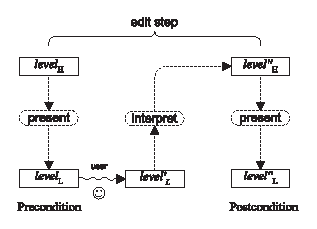
\epsfig{file=pics/eps/LayerSimple.eps, height=1.4in} %width = 60mm}
      \caption{A single edit step.} \label{singleLayerEditFormal}  % visio: Layer.vsd
    \end{center}
\end{figure}

after which the editor computes the final values for the data levels: $level''\L$ and $level''\H$, in order to restore the presentation invariant. Figure~\ref{singleLayerEditFormal} (which was also shown in the previous chapter) illustrates the edit process.

\bc The final higher level is denoted by $level''\H$ rather than $level'\H$ to have a consistent notation for final values. Furthermore, in the multi-layered editor specification (see Section~\ref{sect:compositeExtra}) $level'\H$ will denote the intermediate value for the higher level $level'H$. Figure~\ref{singleLayerEdit} schematically shows the editing process for one edit step. In the rest of this chapter we use the same notation for the different stages of the data levels.

\begin{figure}
\xpr{
level\H 		&   			&		 & 			& level''\H\\
~~~\downarrow &   		&		&~\nearrow~&~~~\downarrow \\
level\L 		&~\leadsto~ & level'\L 	& 			& level''\L\\
}
\caption{Single edit step.(draft)} \label{singleLayerEdit}
\end{figure}


Most likely, after editing, the presentation invariant does not hold between $\level'\L$ and $\level\H$. Hence, we need to find a new higher-level value $\level''\H$. However, because it is possible that $\level'\L$ is not a valid presentation of a higher-level value, we also need to find a new lower level $\level''\L$ in order to restore the presentation invariant. Figure~\ref{} shows the values of the higher and lower levels for the example from the previous section.
\ec 

Besides the presentation invariant, we impose several other requirements on the final levels.

Firstly, if $\level'\L$ is a valid presentation of $\level\H$, we do not want $\level\H$ to change because of the edit operation, and thus $\level''\H = \level\H$. Because, in this section, the presentation mapping is a function, $\level'\L$ can only be a valid presentation of $\level\H$ if it is equal to $\level\L$, meaning that the user did not change the lower level. However, in the next section, when extra state is added to the model, the reason for this property becomes clear. Because the property states that the document stays inert under an edit operation, we refer to it as \law{Doc-Inert}.

Secondly, if a user edits the lower level in such a way that $\level'\L$ is a valid presentation of some higher-level value, then the editor should not perform any further updates on the lower level, and the final value $level''\L$ should be equal $\level'\L$. Analogous to the previous property, this property is referred to as \law{Pres-Inert}.

\bc
Besides \law{Pres-Inert}, we could also add a requirement that if there exists an $h$, such that $level'\L = \present~h$, then $level''\H = h$, since because of \law{Pres-Inert} and injectivity of $\present$, $h$ is the only possible value for $\level''\H$. However, since this requirement will no longer hold in the presence of extra state, we will omit it here as well.
\ec

Our final requirement specifies what happens when $\level'\L$ is not a valid presentation of any higher level. In this case, the editor could simply forbid the edit operation, but a more user-friendly solution is to regard the operation as an inexact edit operation and perform the intended edit operation. This means that the editor chooses a $level''\H$ and $level''\L$ such that $level''\L$ is as close as possible to the $level'\L$ that came from the user (and, of course, $\level''\L = \present~\level''\H$ ).

Summarizing, if we let $Comp$ be a program fragment that assigns new values to the data levels, then the requirements on $Comp$, specified as Hoare triples, are:

\xprlab{\hoare{\true} {Comp} { \level''\L = \present~\level''\H }}{Postcondition}
\xprlab{\hoare{ \level'\L = \present~\level\H } {Comp} { \level''\H = \level\H }}{Doc-Inert}
\xprlab{\hoare{ \level'\L = \present~h } {Comp} {\level'\L = \level''\L}}{Pres-Inert}
\xprlab{\hoare{ \true } {Comp} {\level'\L \close \level''\L}}{Intended}

Note that \law{Pres-Inert} is a special case of \law{Intended}, in which ``close~to'' is equality. In order to prevent a conflict with \law{Postcondition}, \law{Intended} is slightly weaker than \law{Postcondition}.
%\note{Maybe mention precondition more explicitly?} 
%{say that \law{Intended} is weaker} is not true. 


\head{Definition of $Comp$}


A straightforward definition of $Comp$ that meets all requirements is:

\xprlab{
Comp \is 	& \level''\H \gets \interpret~\level'\L \semi\\
				&\level''\L \gets  \present~\level''\H
}{$Comp$-Def}

Together with $Comp$, the requirements above provide a specification of $\interpret$. We can prove that \law{Postcondition} holds, and furthermore, if \law{InterPresent} holds, then \law{Doc-Inert} and \law{Pres-Inert} can be proved as well. \law{Intended} cannot be proved from \law{InterPresent}, and hence is a requirement on $\interpret$ (together with $Comp$).


\head{Basic Hoare logic}

Before we prove the requirements, we introduce a few laws from the Hoare calculus. We use the following law to relate Hoare triples to weakest precondition propositions:

\xprlab{
\hoare{P}{S} {Q} ~\eqv~ P \imp wp(S,Q)
}{\fn{wp}-Char}

Because the program only consists of assignments and a composition, we do not need to consider termination, and moreover, we only need two laws from the weakest precondition calculus. For assignments we have:

\xprlab{
\wp{~x \gets e~}{P} ~\eqv~ P[x/e]\\
}{\fn{wp}-$\gts$}

And a for composition we have:

\xprlab{
\wp{~S \semi T~}{P} ~\eqv~ \wp{S}{ \wp{T}{P} }\\
}{\fn{wp}-$\smi$}

In Section~\ref{sect:compositeExtraEditing} we need two more laws, which we introduce here as well for completeness. We need a law for weakening the postcondition.

\xprlab{
(Q \imp Q') ~\imp~ (\wp{S}{Q} \imp \wp{S}{Q'})\\
}{\fn{wp}-Mono}

\bc
\begin{proof}
assume $Q \imp Q'$
\begin{Prf}&
\true\\
\Eqv{reflexivity of $\imp$}&
wp(S,Q) \imp wp(S,Q)\\
\Eqv{\law{\fn{wp}-Char}}&
\hoare{wp(S,Q)}{S} {Q}\\
\Eqv{Weakening postcondition}&
\hoare{wp(S,Q)}{S} {Q'}\\
\Eqv{\law{\fn{wp}-Char}}&
wp(S,Q) \imp wp(S,Q')\\
\end{Prf}
\end{proof}
\ec

And a law for combining two postconditions.

\xprlab{
(P \imp \wp{S}{Q}) \land (P \imp \wp{S}{Q'}) ~\imp~ (P \imp \wp{S}{Q \land Q'})\\
}{\fn{wp}-And}

\head{\law{Postcondition} requirement}

%\note{Give this proof here? It's rather trivial.}

According to \law{\fn{wp}-Char}, $\hoare{\true} {Comp} { \level''\L = \present~\level''\H }$ is equivalent to:

$\true ~\imp~ \wp{Comp}{ \level''\L = \present~\level''\H }$

\bc Unlike the other proofs in this section, we start the weakest precondition proofs with the antecedent of the implication and work toward the conclusion. This way, the order of the subsitutions in the proof steps corresponds to the evaluation order of the assignment statements in $Comp$. \ec

\begin{proof} 
\begin{Prf}&
	\wp{Comp}{ \level''\L = \present~\level''\H }\\
\Eqv{\law{$Comp$-Def}}&
	\wpWide{\level''\H \gets \interpret~\level'\L \semi \level''\L \gets \present~\level''\H}{ \level''\L = \present~\level''\H } \\
\Eqv{\law{\fn{wp}-$\smi$}}&
	\wpWide{\level''\H \gets \interpret~\level'\L}{ \wp{ \level''\L \gets \present~\level''\H}{ \level''\L = \present~\level''\H }} \\
\Eqv{\law{\fn{wp}-$\gts$}}&
	\wp{\level''\H \gets \interpret~\level'\L}{\present~\level''\H = \present~\level''\H} \\
\Eqv{ reflexivity of $=$ }&
	\wp{\level''\H \gets \interpret~\level'\L}{\true} \\
\Eqv{\law{\fn{wp}-$\gts$}}&
	\true\\
\end{Prf}
\end{proof}

\head{\law{Doc-Inert} requirement}

In the proofs below, we will implicitly use the equivalence between the Hoare notation and the weakest precondition notation suggested by \law{\fn{wp}-Char}. Hence, \law{Doc-Inert} is:

%According to \law{\fn{wp}-Char}, $\hoare{ \level'\L = \present~\level\H } {Comp} { \level''\H = \level\H }$ is equivalent to:

$\level'\L = \present~\level\H ~\imp~ \wp{Comp}{ \level''\H = \level\H}$


\begin{proof} 
\begin{Prf}&
	\wp{Comp}{\level\H = \level''\H}\\
\Eqv{\law{$Comp$-Def}}&
	\wp{\level''\H \gets \interpret~\level'\L \semi \level''\L \gets \present~\level''\H}{\level\H = \level''\H} \\
\Eqv{\law{\fn{wp}-$\smi$}}&
	\wp{\level''\H \gets \interpret~\level'\L}{ \wp{ \level''\L \gets \present~\level''\H}{\level\H = \level''\H}} \\
\Eqv{{\sc \fn{wp}-$\gts$}}&
	\wp{\level''\H \gets \interpret~\level'\L}{\level\H = \level''\H} \\
\Eqv{\law{\fn{wp}-$\gts$}}&
	\level\H = \interpret~\level'\L\\
\Ffr{\law{InterPresent}}&
	\level'\L = \present~\level\H\\
\end{Prf}
\end{proof}

\head{\law{Pres-Inert} requirement}

The proof of \law{Pres-Inert} is similar to the proof of \law{Doc-Inert}

%$\hoare{ \level'\L = \present~h } {Comp} {\level'\L = \level''\L}$, is equivalent to:

$\level'\L = \present~h ~\imp~\wp{Comp}{\level'\L = \level''\L}$ 

\begin{proof}

In the proof, we assume $\level'\L = \present~h$:

\begin{Prf}&
	\wp{Comp}{\level'\L = \level''\L}\\
\Eqv{\law{$Comp$-Def}}&
	\wp{ \level''\H \gets \interpret~\level'\L \semi \level''\L \gets \present~\level''\H}{\level'\L = \level''\L }\\
\Eqv{\law{\fn{wp}-$\smi$}}&
	\wp{\level''\H \gets \interpret~\level'\L}{ \wp {\level''\L \gets \present~\level''\H}{\level'\L = \level''\L} }\\
\Eqv{\law{\fn{wp}-$\gts$}}&
	\wp{\level''\H \gets \interpret~\level'\L}{ \level'\L = \present~\level''\H}\\
\Eqv{\law{\fn{wp}-$\gts$}}&
	\level'\L = \present~(\interpret~\level'\L)\\
\Ffr{assumption} &
	\level'\L = \present~(\interpret~(\present~h))\\
\Eqv{\law{InterPresent}}&
	\level'\L = \present~h \}\\
\end{Prf}
\end{proof}



\head{\law{Intended} requirement}

If $\level'\L$ is not a valid presentation, only \law{Postcondition} and \law{Intended} are of importance:

\xpr{\hoare{ \true } {Comp} {\level'\L \close \level''\L}}

This requirement states that $\interpret$ returns a higher level such that its presentation resembles what the user intended with the edit operation. Because the intention of a user is a rather vague concept, we cannot give a formal specification of the ``close~to'' relation here. It is left to the editor designer to assign a meaning to it and provide an $\interpret$ function that meets the requirement given.

%\note{Is ``close to'' what we want? For simple editors, maybe it is, but is "-$>$" close to \rarr?}
%\note{What about Chapter titles and fonts? Will these be handled correctly with ``close to'' req.?}

%conclusions
% give present, we have two requirements interpresent, intended. and together with $comp$ these specify an editor.




%																
%																
%																
\section{Extra state} \label{sect:singleExtra}

In this section, we extend the specification of the single-layered editor with extra state (see Section~\ref{sect:extraState}). The document level may contain interpretation extra state, whereas the presentation may contain presentation extra state.

In the presence of extra state, a single document may have several presentations, and a single presentation may be the presentation of several documents. This means that we can no longer represent the relation $Present$ by a function $\present$ between values, since $\present~h$ would have to be a set of lower-level levels. Similarly, $\interpret~l$  would have to return a set of higher-level values.

To be able to use functional representations for the presentation and interpretation mappings after all, we introduce an equivalence class representation for extra state. 
Because two levels that only differ in extra state are in a sense equivalent, we model extra state using an equivalence relation on the data level. The elements of an equivalence class are equal except for their extra state. Using this equivalence class representation for extra state, we can express $\present$ and $\interpret$ as set-valued functions between equivalence classes.

%Sections~\ref{sect:editingExtraState} and \ref{sect:extraState} provide examples of extra state, but in order to
%illustrate the equivalence class representation of extra state, we give two simple examples here as well. 
We provide two examples to illustrate the equivalence class representation for extra state. Both examples are set in an editor for a simple programming language, for which layout is not part of the syntax.


\todo{$H$ en $L$ uitleggen}
A partially presented declaration is an example of interpretation extra state. If we hide the right-hand side of a declaration, \verb|Decl "f" (Sum 1 2)| is presented as \verb|f = ...|, which is also a presentation of \verb|Decl "f" (Product 3 4)|. Thus, \verb|(Sum 1 2)| and \verb|(Product 3 4)| are interpretation extra state. If we denote the extra state equivalence relation by $H \tp Level\H \rel Level\H$, we can express this as 
$(\verb|Decl "f" (Sum 1 2)|)~H~(\verb|Decl "f" (Product 3 4)|)$. More generally, a declaration is equivalent to every declaration that has the same left-hand side identifier.

Whitespace is an example of presentation extra state on the lower level. Consider the expression \verb|Sum 1 2|, which is presented as ``{\tt 1\spc+\spc 2}''. The presentation is equivalent to a string containing `\verb|1|', `\verb|+|', and `\verb|2|' with any configuration of whitespace. Thus, for example, 
$``\texttt{1\spc+\spc 2}\text{''}~L~``\texttt{1+2}\text{''}$.


Because no assumptions are made about the types of the two levels, the model for extra state is  rather abstract. Section~\ref{sect:wildcardEq} provides a concrete representation of extra state in tree-structured data types.


%?Next section we give a concrete instance of these classes.

\bc
\bl
\o Simple example a declaration (identifier \& rhs) in a source editor is presented by leaving out the right-hand side:
\o  \verb| (Decl "b" True) <-> "b  =  ..."|\note{or complex expression?}
\o Whitespace is presentation extra state: \verb| (Decl "b" True) -> "*b*=*..."|
\o Right-hand side is interpretation extra state: \verb|b = ... -> (Decl "b" *)|
\el
\ec



\subsection{Equivalence classes}

We start by introducing some notation for equivalence classes. A typed binary relation $R \tp T \rel T$ is an equivalence relation if it is reflexive, symmetric, and transitive.  The equivalence class for a value $x \tp T$ is denoted by $\eqcl{x}{R}$. Its definition is:

\xpr{
%( \eqcl{\hole}{R}) \tp S \to  \Eqcl{S}{R}\\
\eqcl{x}{R} = \setof{y}{x\;R\;y}
}

The factor set $\Eqcl{T}{R}$ is the set of all equivalence classes of $R$. It is a set of mutually exclusive and jointly exhaustive subsets of $T$ (if we regard $T$ as a set).

\xpr{
\Eqcl{T}{R} = \setof{\eqcl{x}{R}}{ x \tp T}
}

We have the following property for an equivalence relation $R$:

\xprlab{
x \in \eqcl{y}{R} ~\eqv~ \eqcl{x}{R} = \eqcl{y}{R}
}{$\eqhole$-Member}


%Proposition:
%\xpr{
%\eqcl{x}{R} = \eqcl{y}{R} ~\lor~ (\eqcl{x}{R} \cap \eqcl{y}{R}) = \emptyset
%}


\subsection{An equivalence class for extra state} \label{sect:eqclassForES}

If several lower-level values are related to the same higher-level value by the presentation relation, this means that when disregarding extra state, the lower-level values are equal. Similarly, if two higher-level values are related to the same lower value, the higher-level values are equal up to extra state. We use an equivalence relation to express that two values are equal up to extra state. 

The two data levels give rise to two equivalence relations: $H$ and $L$.

\xpr{
H \tp Level\H \rel \Level\H~~~~~~\text{and}~~~~~~L \tp Level\L \rel \Level\L\\
}

In order to specify that extra state should be reused after an update, without making any assumptions on the level type, we use the ``close~to'' notion from the previous section. We specify that an updated value $x'$ contains reused extra state from $x$, by requiring that $x'$ is the element of its equivalence class that is as close as possible to $x$. 

As an example, consider an update on the presentation of \verb|Decl "f" (Sum 1 2)| from the example above:  $``\verb|f = ...|\text{''} \leadsto ``\verb|g = ...|\text{''}$. The new higher level should have left-hand side \verb|"g"| and reuse the sum. This can be specified by requiring that from the equivalence class of declarations with left-hand side \verb|"g"|, we select the element that is as close as possible to \verb|Decl "f" (Sum 1 2)|. The obvious solution is \verb|Decl "g" (Sum 1 2)|.



\subsection{Presenting and interpreting}

In the presence of extra state, both the presentation and interpretation mappings may have several results for a single argument, and hence cannot directly be represented by functions anymore. Regarding the mappings as relations (with the levels ordered as in Section~\ref{sect:editProces}), we have:
% they are no longer functions, but binary relations:

\xpr{
Present &\tp& \Level\L \rel \Level\H\\
Interpret &\tp& \Level\H \rel \Level\L
}

%Consequentially, we regard the right ..? as the domain of the relation, and the left .. as the range. 

%\bl
%\o relations are total
%\o say that range is not the set, but only the set for which relation holds
%\el


%\note{maybe say something more about what it means for a relation to be an equivalence class mapping. (Depends non �Composite layer'' section)}


%\note{mention the intuition behind this?  (because arg is also an eq. class, es from one function can never influence result of its dual)}
%Explain that es is classes.
%Present underspecifies lower eq. relation (only on valid). And \interpret is tricky.


\bc
\textdownarrow\textdownarrow\textdownarrow\textdownarrow

Something about what the equivalence classes are: Lower is underspecified: 
PER story

\xpr{
\eqcl{h}{H} = \setof{h'}{\exists l : l~\Present~h \land l~\Present~h'}
}

defines a class on $\Level\H$, since $\Present$ is total, so we have $\eqcl{h}{H}$ for each $h$ on $\Level\H$.

\xpr{
\eqcl{l}{L} = \setof{l'}{\exists h : l~\Present~h \land l'~\Present~h}
}
defines a class on ${\bf range}~\Present \subset \Level\H$, $\Present$ need not be surjective.

$\Interpret$:

\xpr{
\eqcl{h}{H} = \setof{h'}{\exists l : h~\Interpret~l \land h'~\Interpret~l}
}

defines class on $\Level\H$, since $\Interpret$ is total.

Last one is tricky, since also elements without presentation are included in eq. class.
\xpr{
\eqcl{l}{L} = \setof{l'}{\exists h : h~\Interpret~l \land h~\Interpret~l'}
}

Restrict it to range of $\Present$?
That means we would get:

\xpr{
\eqcl{l}{L} = \setof{l'}{\exists h : h~\Interpret~l \land h~\Interpret~l' \land  l'~\Present~h'}
}

\textuparrow\textuparrow\textuparrow\textuparrow
\ec

If we model the extra state on the higher and lower levels with two equivalence relations $H$ and $L$, we can express $Present$ and $Interpret$ as functions between equivalence classes:

\xpr{
\present &\tp& \Eqcl{\Level\H}{H} \rightarrow  \Eqcl{\Level\L}{L}\\
\interpret &\tp& \Eqcl{ \Level\L}{L} \rightarrow \Eqcl{\Level\H}{H}
}


%result is always an eq. class (follows from type)\note{fix $H$ and $L$, since these are the eq. relations, but used %here as sets}
%
%\xpr{
%L = \present~H \imp L = \eqcl{l}{L}\\
%H = \interpret~L \imp H = \eqcl{h}{H}
%}

The correspondence between functions $\present$ and $\interpret$, and relations $\Present$ and $\Interpret$ is made explicit by the two characterizations:

\xprlab{
l~Present~h ~\eqv~ \eqcl{l}{L} = \present~ \eqcl{h}{H}\\
}{\present-Char}
\xprlab{
h~Interpret~l ~\eqv~ \eqcl{h}{H} = \interpret~\eqcl{l}{L}
}{\interpret-Char}

In the remainder of this section, we will use the functional representation.

%\xpr{
%\present~H = \setof{l}{h \in H \land l \in Present~h}
%}



%\head{Presentation invariant}    Seems obsolete now.
%
%\bl
%\o Presentation invariant changes: Works on sets now.
%%\o (\verb|"b = ..."| as well as more spatious \verb|"b    =    ..."| are correct presentations of \verb|Decl "b" True|
%\el
%
%\xprlab{
%\level\L~\Present~\level\H\\
%\text{or, equivalently}\\
%\eqcl{\level\L}{L} = \present~\eqcl{\level\H}{H}
%}{Present}


\head{\law{InterPresent} requirement}

The \law{InterPresent} requirement changes slightly, since we use equivalence class notation to make explicit that the arguments and results are equivalence classes:

\xprlab{
%l~\Present~h \imp h~\Interpret~l\\
%or\\
\eqcl{l}{L} = \present~\eqcl{h}{H} ~\imp~ \eqcl{h}{H} = \interpret~\eqcl{l}{L}\\
}{InterPresent}

Or, equivalently:

\xpr{
\interpret \oo \present = id_{\Eqcl{\Level\H}{H}} 
}

Similar to the previous section, \law{InterPresent} states that $\interpret$ is a left inverse of $\present$ and implies injectivity of $\present$ as well as surjectivity of $\interpret$.

% Kleisli is not applicable anymore. Maybe useful somewhere below.
% old problem with Kleisli:
% l in (pres  `kleisli` int) l       is not True, because that alread holds if there is s single h in int l
% for which l in pres h, but we want for all h in int l that l in pres h



\subsection{Editing} \label{sect:singleExtra_Editing}

Similar to Section~\ref{sect:single_Editing}, we assign new values to the higher and the lower data levels when a user edits the lower level:

\xpr{
\eqcl{\level\L}{L} = \present~\eqcl{\level\H}{H}\\
\level\L \leadsto \level'\L 
}

The old requirements, rewritten with equivalence classes, are:

\xprlab{\hoare{\true} {Comp} { \eqcl{\level''\L}{L} = \present~\eqcl{\level''\H}{H} } }		{Postcondition}
\xprlab{\hoare{\eqcl{\level'\L}{L} = \present~\eqcl{\level\H}{H}} {Comp} { \level\H = \level''\H}}  {Doc-Inert}
\xprlab{\hoare{\eqcl{\level'\L}{L} = \present~\eqcl{h}{H}} {Comp} { \level'\L = \level''\L}}		{Pres-Inert}
\xprlab{\hoare{\true} {Comp} {\level'\L \close \level''\L}}	{Intended}

With extra state, the \law{Doc-Inert} requirement becomes interesting, since it is now possible to update $level\L$ to a (different) $level'\L$, which is still a valid presentation of $level\H$. For example, if whitespace is not stored in the document, and a user edits only whitespace, then the document should remain unchanged.

In addition to the four requirements of the previous section, we need to require that extra state on both levels is reused after an update. For interpretation extra state on the higher level, we require that from the equivalence class specified by \law{Postcondition}, the element  that is as close as possible to the original value $level\H$ is selected:

\xprlab{\hoare{\true} {Comp} {\level\H \close \level''\H}}	{Doc-Preserve}

\law{Doc-Preserve} is weaker than the other requirements. It specifies which element of the equivalence class determined by \law{Postcondition} is the final value of the lower level.

On the lower level, we need a similar requirement for presentation extra state, but here it coincides with \law{Intended}. Thus, \law{Intended} has a double function: it states that the resulting equivalence class of $\present$ must be close to the equivalence class of $level'\L$, as well as that the presentation extra state in $level''\L$ must resemble the extra state in $\level'\L$ as much as possible.


% es part weaker than others, not nec. either not valid, only intended and postcondition. 
% pres of doc, then pres-inert holds, intended does not interfere.  Just valid, same thing.

%\note{do we have to say the \law{Intended} is stronger than \law{Preserve}?}
\head{Reusing extra state}

$Comp$ realizes a mapping between data levels, but both $\present$ and $\interpret$ are mappings between equivalence classes on these data levels. Hence, we need a way to get from values to equivalence classes and back. We use the $\eqhole$ function to denote the equivalence class of a value. For going from an equivalence class to a value, we need a selection function that takes as an extra argument the old value of the level.

The resulting class of $\present$ or $\interpret$ contains all possible extra state configurations.
From this class, we need to select an element for which the extra state resembles the extra state of the previous value as much as possible. Thus, we introduce the function $\reuz \tp  \Eqcl{X}{R} \to X \to X$, which takes an equivalence class and a previous value, and selects the element from the class that is closest to the previous value. Intuitively,~$\reuz$ ``reuses'' the extra state from the previous value.  In this section, we will only give a number of requirements for $\reuz$. Section~\ref{sect:wildcardEq} provides a more concrete instance. 

%The type of~$\reuz$ is:
%\xprlab{
%\reuz \tp  \Eqcl{X}{R} \to X \to X\\
%}

Because we need to reuse extra state on the results of $\present$ as well as $\interpret$, we need two $\reuz$ functions: one for each level. In order to disambiguate between the two functions, we add the corresponding relation as a subscript (e.g.\ $\reuze{H}$ and $\reuze{L}\!$). For the higher level we have $\reuze{H} \tp  \Eqcl{Level\H}{H} \to Level\H \to Level\H$, and for the lower level $\reuze{L} \tp  \Eqcl{Level\L}{L} \to Level\L \to Level\L$

We require several properties of~$\reuz$. First of all, the equivalence class that is the result of~$\reuz$ must be equal to the argument equivalence class:

%\xprlab{\eqcl{x}{R} \reuz y \in \eqcl{x}{R}}				{$\reuz$-Valid}
\xprlab{\eqcl{\eqcl{x}{R} \reuz y}{R} = \eqcl{x}{R}}	{$\reuz$-Valid}

Furthermore, if the value argument is in the equivalence class argument, then~$\reuz$ returns the value argument.

 
%\xprlab{y \in \eqcl{x}{R} \imp \eqcl{x}{R} \reuz y = y}			{$\reuz$-Idem} 
\xprlab{\eqcl{y}{R} = \eqcl{x}{R} ~\imp~ \eqcl{x}{R} \reuz y = y}	{$\reuz$-Idem} 

Note that, by \law{$\reuz$-Valid}, we also have the reverse: $\eqcl{x}{R} \reuz y = y ~\imp~ \eqcl{y}{R} = \eqcl{x}{R} $.\nonote{is \law{$\reuz$-Valid} implied by  equivalence version of \law{$\reuz$-Idem}?}

Finally, if the value argument is not in the equivalence class argument, then~$\reuz$ returns an element of that class that is as close as possible to the value argument.

\xprlab{\eqcl{x}{R} \reuz y \close y}		{$\reuz$-Close} 

Similar to the \law{Doc-Inert} and \law{Intended} requirements, \law{$\reuz$-Idem} is a special case of \law{$\reuz$-Close}, for which ``close~to'' is equality.

\head{Definition of $Comp$}

Using $\eqcl{\hole}{}$ and $\reuz$ we can define $Comp$. The definition is split in $Up$ and $Dwn$ to make the proofs of the requirements more readable. %(will be split for composite layers anyway).

%\xprlab{
%\level''\H = \interpret~ \eqcl{\level'\L}{L}  ~\reuze{H}~   \level\H  \\ %(\level'\L,\level\H)\\ 
%\level''\L = \present~ \eqcl{\level''\H}{H}   ~\reuze{L}~   \level'\L % ^* (\level''\H, level'\L)
%}{Compute}
%\xprlab{
%Comp \is 	& \level''\H = \interpret~ \eqcl{\level'\L}{L}  ~\reuze{H}~   \level\H \semi\\
%				& \level''\L = \present~ \eqcl{\level''\H}{H}   ~\reuze{L}~   \level'\L
%}{$Comp$-Def}

\xprlab{
Comp \is 	& Up \semi Dwn}{$Comp$-Def}
\xprlab{
Up \is		& \level''\H \gets \interpret~ \eqcl{\level'\L}{L}  ~\reuze{H}~   \level\H}{$Up$-Def}
\xprlab{
Dwn \is		& \level''\L \gets \present~ \eqcl{\level''\H}{H}   ~\reuze{L}~   \level'\L}{$Dwn$-Def}

Similar to the previous section, we can prove that $Comp$ meets the \law{Postcondition}, and, if we assume \law{InterPresent}, also \law{Doc-Inert} and \law{Pres-Inert}. 

\head{\law{Postcondition} requirement}

%Because of \law{\fn{wp}-Char}, \law{Postcondition} is equivalent to:
The weakest precondition notation of \law{Postcondition} is:

$\true ~~\imp~~\wp{Comp}{\eqcl{\level''\L}{L} = \present~\eqcl{\level''\H}{H}}$

\begin{proof} 
\begin{Prf}&
	\wp{Comp}{\eqcl{\level''\L}{L} = \present~\eqcl{\level''\H}{H}}\\
\Eqv{\law{$Comp$-Def}}&
	\wp{Up \semi Dwn}{ \eqcl{\level''\L}{L} = \present~\eqcl{\level''\H}{H} }\\
\Eqv{\law{\fn{wp}-$\smi$}}&
	\wp{Up}{ \wp{Dwn }{ \eqcl{\level''\L}{L} = \present~\eqcl{\level''\H}{H} }}\\
\Eqv{\law{$Dwn$-Def}}&
	\wpWide{Up}{ \wp{\level''\L \gets \present~ \eqcl{\level''\H}{H}   ~\reuze{L}~   \level'\L}{ \eqcl{\level''\L}{L} = \present~\eqcl{\level''\H}{H} }}\\
\Eqv{\law{\fn{wp}-$\gts$}}&
	\wp{Up}{ \eqcl{\present~ \eqcl{\level''\H}{H}   ~\reuze{L}~   \level'\L}{L} = \present~\eqcl{\level''\H}{H}  }\\
\Eqv{ \law{$\reuz$-Valid} }&
	\wp{Up}{ \present~ \eqcl{\level''\H}{H} = \present~\eqcl{\level''\H}{H}  }\\
\Eqv{ reflexivity of~$=$ }&
	\wp{Up}{ \true }\\
\Eqv{\law{$Up$-Def}}&
	\wp{\level''\H \gets \interpret~ \eqcl{\level'\L}{L}  ~\reuze{H}~   \level\H}{  \true  }\\
\Eqv{\law{\fn{wp}-$\gts$}}&
	 \true  \\
\end{Prf}
\end{proof}

\head{\law{Doc-Inert} requirement}

%$\hoare{\eqcl{\level'\L}{L} = \present~\eqcl{\level\H}{H}} {Comp} { \level\H = \level''\H }$

$\eqcl{\level'\L}{L} = \present~\eqcl{\level\H}{H} ~~\imp~~ \wp{Comp}{\level\H = \level''\H}$

\begin{proof}

\begin{Prf}&
	\wp{Comp}{\level\H = \level''\H}\\
\Eqv{\law{$Comp$-Def}}&
	\wp{Up \semi Dwn}{ \level\H = \level''\H }\\
\Eqv{\law{\fn{wp}-$\smi$}}&
	\wp{Up}{ \wp{Dwn }{ \level\H = \level''\H }}\\
\Eqv{\law{$Dwn$-Def}}&
	\wp{Up}{ \wp{\level''\L \gets \present~ \eqcl{\level''\H}{H}   ~\reuze{L}~   \level'\L}{ \level\H = \level''\H }}\\
\Eqv{\law{\fn{wp}-$\gts$}}&
	\wp{Up}{ \level\H = \level''\H }\\
\Eqv{\law{$Up$-Def}}&
	\wp{\level''\H \gets \interpret~ \eqcl{\level'\L}{L}  ~\reuze{H}~   \level\H}{ \level\H = \level''\H }\\
\Eqv{\law{\fn{wp}-$\gts$}}&
	\level\H = \interpret~ \eqcl{\level'\L}{L}  ~\reuze{H}~   \level\H \\
\Ffr{\law{$\reuz$-Idem}}&
	\eqcl{\level\H}{H} = \interpret~\eqcl{\level'\L}{L} \\
\Eqv{\law{InterPresent}}&
	\eqcl{\level'\L}{L} = \present~\eqcl{\level\H}{H}\\
\end{Prf}
\end{proof}


\head{\law{Pres-Inert} requirement}

%$\hoare{\eqcl{\level'\L}{L} = \present~\eqcl{h}{H}} {Comp} { \level'\L = \level''\L}$
%We prove \law{Pres-Inert} by proving the equivalent:

$\eqcl{\level'\L}{L} = \present~\eqcl{h}{H} ~~\imp~~ \wp{Comp}{ \level'\L = \level''\L  }$

\begin{proof}

We assume $\eqcl{\level'\L}{L} = \present~\eqcl{h}{H}$.
	
\begin{Prf}&
	\wp{Comp}{ \level'\L = \level''\L  }\\
\Eqv{\law{$Comp$-Def}}&
	\wp{Up \semi Dwn}{ \level'\L = \level''\L  }\\
\Eqv{\law{\fn{wp}-$\smi$}}&
	\wp{Up}{\wp{Dwn}{ \level'\L = \level''\L  }}\\
\Eqv{\law{$Dwn$-Def}}&
	\wp{Up}{\wp{\level''\L \gets \present~ \eqcl{\level''\H}{H}   ~\reuze{L}~   \level'\L}{ \level'\L = \level''\L  }}\\
\Eqv{\law{\fn{wp}-$\gts$}}&
	\wp{Up}{\level'\L = \present~ \eqcl{\level''\H}{H}   ~\reuze{L}~   \level'\L }\\
\Eqv{\law{$Up$-Def}}&
	\wpWide{\level''\H \gets \interpret~ \eqcl{\level'\L}{L}  ~\reuze{H}~   \level\H}{\level'\L = \present~ \eqcl{\level''\H}{H}   ~\reuze{L}~   \level'\L }\\
\Eqv{\law{\fn{wp}-$\gts$}}&
	\level'\L = \present~ \eqcl{\interpret~ \eqcl{\level'\L}{L}  ~\reuze{H}~   \level\H}{H}   ~\reuze{L}~   \level'\L\\
\Eqv{assumption}&
	\level'\L = \present~ \eqcl{(\interpret~(\present~\eqcl{h}{H})  ~\reuze{H}~  \level\H)}{H}   ~\reuze{L}~  \level'\L\\
\Eqv{\law{InterPresent }}&
	\level'\L  = \present~ \eqcl{(\eqcl{h}{H}  ~\reuze{H}~   \level\H)}{H}   ~\reuze{L}~   \level'\L\\
\Eqv{\law{$\reuz$-Valid}}&
	\level'\L  = \present~\eqcl{h}{H}  ~\reuze{L}~  \level'\L\\
\Eqv{assumption}&
	\level'\L  = \eqcl{\level'\L}{L}~\reuz~  \level'\L\\
\Eqv{ \law{$\reuz$-Idem} }&
	\eqcl{\level'\L}{L} = \eqcl{\level'\L}{L}\\
\Eqv{reflexivity of $=$}&
	\true\\
\end{Prf}
\end{proof}



\head{\law{Doc-Preserve} and \law{Intended} requirements}

For the \law{Doc-Preserve} and \law{Intended} requirements, we give an informal argumentation because of the informal nature of the \close requirement. 

From \law{$Up$-Def}, we know that $level''\H$ is the result of  $\interpret~ \eqcl{\level'\L}{L}  ~\reuze{H}~   \level\H$, which implies $level\H \close level''\H$ by \law{$\reuz$-Close}. Hence, \law{Doc-Preserve} holds.

The \law{Intended} requirement is somewhat more subtle, since it has a double function. On the one hand, it states that the equivalence class $\eqcl{\level''\L}{L}$ must be close to $\eqcl{\level'\L}{L}$. This corresponds to the \law{Intended} requirement in Section~\ref{sect:single_Editing} without extra state. In this sense, closeness is used to express that the final lower level resembles what the user intended. Thus, if $level'\L$ is not a valid presentation, then $\eqcl{level''\H}{H}$, must be chosen such that its presentation equivalence class $\eqcl{\level''\L}{L}$ is close to $\eqcl{\level'\L}{L}$. This part of the requirement is therefore a specification of $\interpret$.


On the other hand, \law{Intended} also states that from the equivalence class $\eqcl{\level''\L}{L}$,
%$\present \eqcl{level''\H}$
 we want to choose an element that is as close as possible to $level'\L$ regarding its extra state. This closeness is guararanteed by \law{$\reuz$-Close} in the same way as on the higher level for \law{Doc-Preserve}.





%																
%																
%																
\section{A wildcard representation for equivalence classes} \label{sect:wildcardEq}

In this section, we give a representation for equivalence classes for a simple kind of tree data structures. We introduce a wildcard notation for representing extra state. Furthermore, we provide an instance of the reuse function ($\reuz$), specific to wildcard values.

% now only trees, still enough. non tree also works if isomorphic.

The specification for reusing extra state is a first step, and needs to be extended further to allow reusing extra state for more edit operations. The final subsection sketches such an extension.



% Notes:
%
% $pres n = n `div` 2$ is no longer possible, since eq. classes on pres are 
% then $\set{\set{0,1},\set{2,3}, \dots }$, for which there is no * rep. (0 and 1 in eq. class implies all elts in eq. class)
% can we handle $\set{ {\tt "return\spc1" },{\tt "return\spc\spc1" }, {\tt "return\spc\spc\spc1" }, \dots}$?
%Yes, maybe use an isomorphic view 

\subsection{Trees with wildcards} \label{sect:treesWildcards}
% types are $$ because Int, Bool etc. are used also in a non-Haskell sense
% constructors are \tt
% C constructors are meta-constructors  (and T is type var.)

In a tree-structured data type, we can model extra state by leaving certain parts of the tree undetermined. We do this by representing each extra state-part by a wildcard, which stands for any possible value of the correct type. The functions $\present$ and $\interpret$ return a value that contains wildcards, thus leaving the extra state in the result undetermined.

For a type $T$, the corresponding wildcard is denoted by  $\texttt{*}_{T}$ and has type $*_T$ (note the different font):

\xpr{
\data~*_T  = \texttt{*}_{T}\\
}
 
The wildcard for type $T$ represents any possible value of type $T$. Thus, the value $\texttt{*}_{Bool}$ represents any value from the set $\set{{\tt True}, {\tt False}}$, and the value $\texttt{*}_{Int}$ represents any integer. An example shows how wildcards can be used to model extra state equivalence classes in a data type.

%explain diff between type $*$ and value for $\texttt{*}$

Consider a simple binary tree data type:

\xpr{
\data~Tree  = {\tt Bin}~Bool~Tree~Tree~|~{\tt Leaf}~Bool~Int\\
}


We can recursively define a type $Tree^*$ in which we specify for each child type whether or not it is extra state. If, for example, we wish to declare the boolean in the \p{Bin} node and the integer in the \p{Leaf} as extra state, we represent these children by wildcards:

\xpr{
\data~Tree^*  = {\tt Bin}~*_{Bool}~Tree^*~Tree^*~|~{\tt Leaf}~Bool^*~*_{Int}\\
}

Note that for a type without children, such as \p{Bool}, the wildcard type is the same as the original type ($\p{Bool}^*=\p{Bool}$). Nevertheless, for uniformity, we replace every child type $T$  by a type $T^*$, even if $T$ has no children.

For simplicity, the constructors for type $T^*$ are the same as for $T$. A sample value of type $Tree^*$ is:
 ${\tt Bin} ~\texttt{*}_{Bool}~ ({\tt Leaf~True}~\texttt{*}_{Int})~({\tt Leaf~False}~\texttt{*}_{Int})$. 
 
% mention that * are terms

For a type $T$, a type $T^*$ specifies which parts of it are extra state. Note that for a single type $T$ several types $T^*$ are possible: whether or not a value is extra state is not determined by its type, but rather by the $T^*$ declarations in which  the value appears as a child. In the example, a boolean in a ${\tt Bin}$ node is extra state, whereas a boolean in a ${\tt Leaf}$ is not. The editor designer specifies which parts of a $Level$ type are extra state by declaring an appropriate $Level^*$.

Because a wildcard represents the set of all possible values of a certain type, a value containing a wildcard also represents a set of values. A value that contains several wildcards also represents the set that is formed by taking all possible combinations of values for the wildcards.

We use the notation $\para{x}$ for the set of values represented by a value $x \tp T^*$. Thus,  $\para{\texttt{C~*}_{Bool} \texttt{*}_{Bool}} = \set{{\tt C~True~True}, {\tt C~True~False}, {\tt C~False~True}, {\tt C~False~False}}$.

In order to obtain a $T^*$ value for a value of type $T$, we define a function $\core \tp T \to T^*$, which drops all information that is masked by a wildcard in the $T^*$ definition. For example, for the type definition $\mathbf{data}~T^* = \texttt{T}~Int~*_{Bool}$, we have $\core~(\texttt{T}~1~\texttt{True}) = \texttt{T}~1~\texttt{*}_{Bool}$.

The root of the document cannot be extra state, because it is not a child of any constructor. Even though it is unlikely that we want the root to be extra state, it may still be declared as such by using a dummy root type $\data~R = {\tt R}~Root$, and declare the $Root$ child as extra state: $\data~R^* = {\tt R}~*_{Root}$.  

In general, we regard a recursive first-order Haskell data type $T$ as:

% C is var
\xpr{
\data~T  =  \p{C}_0~T_{0,0} \dots T_{0,m_0} ~|~ \dots ~|~ \p{C}_n~T_{n,0} \dots T_{n,m_n} \\
}

We can specify which parts of $T$ are extra state by defining a wildcard type $T^*$. In the definition of $T^*$, we specify for each child of each constructor of $T$ whether or not is extra state. Thus, for constructor $\p{C}_i$, child number $j$ is either $T^*_{i,j}$ or $*_{T_{i,j}}$.

%\xpr{\data~T^* =  \p{C}_0~U_{0,0} \dots U_{0,m_0} ~|~ \dots ~|~ \p{C}_n~U_{n,0} \dots U_{n,m_n}\\ 
%\text{with}~ U^*_{i,j} = T^*_{i,j}
%}

\xpr{\data~T^*~&=& ~\p{C}_0~(T^*_{0,0} \text{~or~} *_{T_{0,0}}) ~\dots~ (T^*_{0,m_0} \text{~or~}*_{T_{0,m_0}})\\
 &\;|&~ \dots\\ 
 &\;|&~ \p{C}_n~(T^*_{n,0} \text{~or~} *_{T_{n,0}}) ~\dots~ (T^*_{n,m_n} \text{~or~} *_{T_{n,m_n}})\\ 
}


%We define  $\para{x}$ to be the set of values represented by a value $x \tp T^*$. Thus, for example,  $\para{ \p{C} %\texttt{*}_{Bool} \texttt{*}_{Bool}} = \set{{\tt \p{C}~True~True}, {\tt \p{C}~True~False}, {\tt \p{C}~False~True},{\tt %\p{C}~False~False}}$

If we use the notation $\powerset~T$ for the power set of $T$, the definition of $\para{\hole}$ is:

\xprlab{
\para{\hole} \tp T^* \to \powerset~T\\
\para{*_ T} \eq \setof{x}{x \tp T}\\
\para{\p{C}~x^*_0 \dots x^*_n} \eq \setof{ \p{C}~x_0 \dots x_n}{x_0 \in \para{x^*_0} \land \dots  \land x_n \in \para{x^*_n}} 
}{$\para{\hole}$-Def}


%In order to obtain a $T^*$ value for a value of type $T$, we define the function $\core \tp T \to T^*$, which drops all information %in a value that is masked by a $*$ in the type definition $T^*$. For example, for a type definition $\mathbf{data}~T^* = %\texttt{T}~Int~*_{Int}$, we have $\core~(\texttt{T}~1~\texttt{True}) = \texttt{T}~1~\texttt{*}_{Bool}$

And the definition of $\core$ is:

 \xprlab{
{\bf data}~T^* = \dots ~|~ \p{C}_i~U_{i,0} \dots U_{i,m_i} ~|~ \dots
~~~~(\text{with}~ U_{i,j} = T^*_{i,j} \text{~or~} *_{T_{i,j}})\\
\\  
\core \tp T \to T^*\\
\core~(\p{C}_i~x_0 \dots x_{m_i}) \eq \p{C}_i~x'_0 \dots x'_{m_i} \\
{\bf where}~ x'_j = \left\{
\begin{array}{ll}
\texttt{*}_{T_{i,j}} & ,~ {\bf if}~ U_{i,j} = *_{T_{i,j}}\\
\core~x_j & ,~ {\bf otherwise}
\end{array}\right.
}{$\core$-Def}


%Note that unlike $\para{\hole}$, $\core$ depends on the definition of $T^*$; different wildcard types give rise to different $\core$ %functions.

%% statement below was for * types with * alternative for each constructor. Does not hold for the new * types
%Because the constructors are the same, converting a value in $T$ to a value in $T*$ is trivial.
%any value of $T$Same constructor, therefore all vals of T are also values of $T^*$


\subsection{$T^*$ induces an equivalence relation on $T$}

We can define two values of type $T$ to be equivalent when they are equal, or only differ in extra state. The resulting binary relation on $T$ is denoted by $\eqstar~\tp T \rel T$. For the definition of $\eqstar$ we use the function $\core$, which is uniquely determined by $T^*$:

\xprlab{
%\setof{ x \eqstar y}{  x \in \para{x^*} \land y \in \para{y^*} \land x^* = y^*}
x \eqstar y \is  \core~x = \core~y
}{$\eqstar$-Def}

To see that $\eqstar$ is an equivalence relation, we need the theorem below, the simple proof of which has been omited:

\xpr{
\text{``$R$~is an equivalence relation''}~~\eqv~~\exists f : \forall x,y : x\;R\;y ~\eqv~ (f~x = f~y)
}

By substituting $\core$ for $f$ and $\eqstar$ for $R$ in this theorem, we can immediately conlude that $\eqstar$ is an equivalence relation on $T$. 

Without giving a proof, we mention that the equivalence classes of $\eqstar$ can be expressed using $\para{\hole}$ and $\core$. 

\xprlab{
\eqcl{x}{\eqstar} \eq \para{\core~x}
}{$\eqstar$-Classes}
\bc
This one was already proven:

\xpr{
(\exists f : x\;R\;y ~\eqv~ (f~x = f~y) ~\imp~ R~\text{is an equivalence relation}
}


\begin{proof} \note{maybe leave this out, or prove equiv. See how much space/time we have}
\begin{Prf}&
x\;R\;x 	& \Eqv{definition of $R$}\\
f x = f x 	& \Eqv{reflexivity of =}\\
\true\\
\end{Prf}


\begin{Prf}&
x\;R\;y  	& \Eqv{definition of $R$}\\
f x = f y 	& \Eqv{symmetry of =}\\
f y = f x 	& \Eqv{definition of $R$}\\
y\;R\;x\\
\end{Prf}\note{get $\eqv$ instead of $\imp$}

\begin{Prf}&
x\;R\;y  \land y\;R\;z 		& \Eqv{definition of $R$}\\
f x = f y \land f y = f z	& \Imp{transitivity of =}\\
f x = f z 				& \Eqv{definition of $R$}\\
x\;R\;z\\
\end{Prf}
\end{proof}
\ec

\subsection{Reuse on wildcard types}\label{subsect:defReuseStar}

We use wildcard types to represent the results of $\present$ and $\interpret$.  Because each wildcard represents a set of values, we need to select an element from each of these sets to obtain a final value for the result. This selection corresponds to filling in a value of type $T$ for each wildcard $\texttt{*}_{T}$ in the result. The values that are filled in for the wildcards are taken from the previous value of the level, if possible.

In this section, we define a function $\reuzestar$ that fills in the wildcards in its first argument by reusing values from its second argument. The type of $\reuzestar$ is:

\xpr{
\reuzestar ::  T^* \to T \to T\\
}

%The property that the parts of a value that are not extra state are maintained can be stated as $x^* \reuzestar y = \core~x^*$. 

We give two examples to show how $\reuzestar$ is used.

Consider a $Token$ data type with a presentation extra state tuple to denote the whitespace. If a token for \verb|"False"| with a whitespace of one linebreak and three spaces is updated to a token \verb|"True"|, then the whitespace of the old token is reused by $\reuzestar$:

$(\verb|Token |\texttt{*}_{(Int, Int)} \verb| "True"|) \reuzestar  (\verb|Token (1,3) "False"|) \eq \verb|Token (1,3) "True"|$

For the second  example, we take the declaration with the hidden right-hand side from Section~\ref{sect:eqclassForES}: \verb|Decl "f" (Sum 1 2)|. If a user renames the left-hand side in the presentation to \verb|g|, the result of $\interpret$ contains the new identifier \verb|"g"|, but the right-hand side is interpretation extra state and will be a $\texttt{*}_{Exp}$. Again, $\reuzestar$ recovers the extra state from the previous value: 

$(\verb|Decl "g" |\texttt{*}_{Exp}) \reuzestar  (\verb|Decl "f"  (Sum 1 2)|) \eq \verb|Decl "g" (Sum 1 2)|$

In some cases, reusing extra state from a previous value is not possible. For example, when a new subtree is inserted in a level, its extra state will not be present in the previous value of the level. Furthermore, if a level is structurally changed, even if all extra state is present in the previous value, it may not always be possible to recover it. In case extra state cannot be reused, we use a function to obtain a default value: $\default \tp a^* \rightarrow a$.

We give a $\default$ function for the declaration example. If a new declaration is inserted, its hidden right-hand side is initialized to the special expression \texttt{Undefined}.

\xprlab{
\default~(\texttt{Decl}~i~e) = \left\{
\begin{array}{ll}
 \texttt{Decl}~i~\texttt{Undefined} & , {\bf if}~ e = \texttt{*}_{Exp} \\
\texttt{Decl}~i~e & , {\bf otherwise}
\end{array}\right.
}

We require that the result of $\default$ is equal to its argument, except for the wildcards in the argument. Wildcards are replaced by default values.

\xprlab{
\default~x^* \in \para{x^*}\\
}{$\default$-Valid}

Because $\default \tp T^* \rightarrow T$ strongly depends on type $T$, we cannot give a general definition of the function. However, it will generally have this pattern:

\xprlab{
\default~\texttt{*}_T = \text{default value for type $T$}\\
\default~(\p{C}~x^*_0 \dots x^*_n) = \p{C}~(\default~x^*_0) \dots (\default~x^*_n) \\
}

The definition is just a sketch, because it suggests that the default for a value only depends on its type, whereas values of the same type that appear in different places may have different defaults. In the  $\default$ for declarations, as defined above, a $\texttt{*}_{Exp}$ wildcard appearing in a \texttt{Decl} gets the default value \texttt{Undefined}, but in other places the default may be different.

%For example, if whitespace is represented by a tuple of integers for line-breaks and spaces, then the algorithm above suggests that %the default for both integers is the same.

Another difficulty in giving a general definition of $\default$ is that a default value may also depend on information elsewhere in the tree, for example when default whitespace is computed by a pretty-printing algorithm. In that  case, the $\default$ function requires an extra argument containing the context of the subtree that is to be pretty-printed.

Using $\default$ we can give a first definition of $\reuzestar$. It takes a new value containing wildcards, together with an old value, and returns the new value with extra state from the old value.

\xprlab{
\texttt{*}_T ~\reuzestar~  y \eq y\\
\p{C}~x^*_0 \dots x^*_n ~\reuzestar~ \p{C}~y_0 \dots y_n \eq \p{C}~(x^*_0 \reuzestar y_0) \dots (x^*_n  \reuzestar y_n) \\
\p{C}~x^*_0 \dots x^*_n ~\reuzestar~ \p{C}'~y_0 \dots y_m \eq \default~(\p{C}~x^*_0 \dots x^*_n)
%~~~~~~~(\text{with~}\p{C} \neq \p{C}')
}{$\reuzestar$-Def}

This is only a basic definition of $\reuzestar$ that recovers extra state only if the old and the new value are structurally similar. If the constructors for the two values are different, a default value is chosen for extra state. Although sufficient for some cases, this method of reusing, based on structure only, is too coarse in general.

Consider an element that is deleted from a list (e.g.\ $[e_0, e_1] \leadsto [e_1]$). A structure-based reuse will recover extra state from $e_0$ for the new value $e_1$, which is not the desired behavior. Similarly, when swapping child nodes in a tree, the extra state will not swap. And finally, when a subtree is updated to a structurally similar subtree, such as 
$\verb|Sum|~e_1~e_2 \leadsto \verb|Product|~e_1~e_2$, we might want the extra state of the children to be reused, which is not possible with this basic $\reuzestar$.

We can handle the problems mentioned above by extending the model with a notion of subtree identities, and defining a more powerful reuse function. Section~\ref{subsect:reuseid} sketches how such a function may be defined.


\subsection{Reuse on equivalence classes} \label{sect:defReuse}

The reuse function $\reuzestar$ defined in the previous section takes a wildcard argument of type $T^*$, whereas the reuse function required for $Comp$ in Section~\ref{sect:singleExtra_Editing} takes an equivalence class argument. Because a wildcard type definition induces an equivalence relation, we can use $\reuzestar$ for $\reuz$. However, since not every equivalence relation has a wildcard representation, we thus put a restriction on the equivalence relations that we can define on the results of $\present$ and $\interpret$, and hence on the kind of extra state we can model.

Recall the types of $\present$ and $\interpret$:

\xprlab{
\present &\tp& \Eqcl{\Level\H}{H} \rightarrow  \Eqcl{\Level\L}{L}\\
\interpret &\tp& \Eqcl{\Level\L}{L} \rightarrow  \Eqcl{\Level\H}{H}
}

%We assume that the equivalence relations $H$ and $L$ are implied by wildcard types $\Level^*\H$ and $\Level^*\L$. This %gives rise to  Hence:
%explain bit more, two or more implies all. also for constructor.\note{comment probably obsolete}

A wildcard type $\Level^*\H$ induces an equivalence relation $\eqstar$ and the corresponding $\core$ and $\reuzestar$ functions. We restrict ourselves by requiring that the extra state on $\Level\H$ has a wildcard representation. Thus, we require the existence of a $\Level^*\H$, such that $H \eqv {\eqstar}$. A similar restriction applies to the lower level.

To disambiguate instances of $\core$ for the different levels, we use subscripts H and L (rather than the verbose $\Level^*\H$ and $\Level^*\H$).  The equivalence classes on the higher and lower levels can be expressed as: 

\xprlab{
h\;H\;h'	&\is	&\core\!\H~h = \core\!\H~h'\\
l\;L\;l' 	&\is	&\core\!\L~l = \core\!\L~l'\\
%\eqcl{h}{H} \eq \para{ \core_{\!H}~h}_{\!_{H}}\\
%\eqcl{l}{L} \eq \para{ \core_{\!L}~l}_{\!_{L}}\\
}{Restrict}

%A wildcard type $\Level^*\H$ induces an equivalence relation $\eqstar_{\rm H}$ and corresponding $\core_{\rm H}$, and %$\reuzestar_{\rm H}$ functions. Similarly, a type $\Level^*\L$ gives rise to a relation $\eqstar_{\rm H}$ and corresponding %functions. 
%
%We now restrict ourselves by requiring that the extra state on $\Level\H$ and $\Level\L$ has a wildcard representation. Thus, we %require the existence of a $\Level^*\H$ and a $\Level^*\L$, such that $H \eqv {\eqstar_{\rm H}}$ and
%$L \eqv {\eqstar_{\rm L}}$. The equivalence classes on the higher and lower level can therefore be expressed in terms of %$\para{\hole}$ and $\core$:
%
%\xprlab{
%\eqcl{h}{H} \eq \para{ \core_{\rm H}~h}\\
%\eqcl{l}{L} \eq \para{ \core_{\rm L}~l}\\
%}{Restrict}


Because the results in the remainder of this section apply to either level, we drop the subscripts to $\core$ and other level-specific functions. We use $R$ to denote either relation $H$ or $L$. Thus, from \law{$\eqstar$-Classes}, we have:

\xprlab{
\eqcl{x}{R} \eq \para{\core~x}
}{Restrict-Classes}

%For $x$ of type $T$, we assume that there is a $T^*$ wildcard type, let $\eqsim$ be the equivalence class 

%\xprlab{
%\eqclass{x}{\eqstar} \eq \para{ \core~x}
%}{Restrict}% deze weg doen?


We define $\reuz$ in terms of $\reuzestar$:

\xprlab{
\reuz ::  \Eqcl{T}{R} \to T \to T\\
\eqcl{x}{R} \reuz y \is \core~x \reuzestar y 
}{$\reuz$-Def}

%\note{maybe mention that we cannot use this one on composition eq. classes}

In order for this definition to be valid, we have to verify that it returns the same result for all elements in an equivalence class.

\xpr{
x\;R\;x'  ~~\imp~~ \eqcl{x}{R} \reuz y \equ \eqcl{x'}{R} \reuz y
}
\begin{proof}
\begin{Prf}&
	\eqcl{x}{R} \reuz y \equ \eqcl{x'}{R} \reuz y\\
\Eqv{$\reuz$-Def}&
	\core~x \reuzestar y \equ \core~x' \reuzestar y\\ 
\Ffr{Leibniz}&
	\core~x \equ \core~x'\\
%	\para{ \core~x}_{\!_{R}} \equ \para{\core~x'}_{\!_{R}}\\
\Eqv{\law{Restrict}}&
	x\;R\;x'\\
\end{Prf}
\end{proof}


Before we prove that  $\reuz$ meets  the \law{$\reuz$-Valid}, \law{$\reuz$-Idem}, and  
\law{$\reuz$-Close} requirements from Section~\ref{sect:singleExtra_Editing}, we introduce a more uniform wildcard type that will simplify the proofs.

\head{The $T\st$ type}

The structure of a wildcard type definition $T^*$ leads to awkward proofs, because each child of a constructor can be either a wildcard or a regular child. When pattern matching, this means that children cannot be handled uniformly. Therefore, we introduce a uniform construction assigning a data type $T\st$, which has an extra wildcard constructor, to every type $T$, including the primitive types. 
(Note the different star symbols: `$\star$' for the uniform type versus `$*$' for the regular wildcard type.) 

For a type $T$:

\xpr{
\data~T  =  \p{C}_0~T_{0,0} \dots T_{0,m_0}~|~\dots~|~\p{C}_n~T_{n,0} \dots T_{n,m_n} \\
}

we can construct a data type $T\st$ by:

\xpr{
\data~T\st =  \p{C}_0~T\st_{0,0} \dots T\st_{0,m_0} ~|~\dots~|~\p{C}_n~T\st_{n,0} \dots T\st_{n,m_n}~|~\texttt{*}_T\\
}

For the binary tree from~\ref{sect:treesWildcards}, we get:

\xpr{
\data~Tree\st  = {\tt Bin}~Bool\st~Tree\st~Tree\st~|~{\tt Leaf}~Bool\st~Int\st~|~\texttt{*}_{Tree}\\
}

Note that the construction also applies to the primitive types $Bool$ and $Int$, and extends these types with a wildcard constructor. Hence, the possible values for the type $Bool\st$ are: $\texttt{True}$, $\texttt{False}$, and $\texttt{*}_{Bool}$.


%A $T^*$ type can be viewed as an inlined version of a $T\st$ type.  
Unlike $T^*$ types, a data type $T$ has only one $T\st$ type. Because $T^*$ and $T\st$ share the $\texttt{*}_T$ constructor, any $T^*$ value is also a $T\st$ value. For example, for the type $Tree^*$ from Section~\ref{sect:treesWildcards}, we have 
${\tt Leaf~True}~\texttt{*}_{Int}\tp Tree^*$ as well as ${\tt Leaf~True}~\texttt{*}_{Int}\tp Tree\st$. 
Because the constructors are shared, the functions $\reuzestar$ and $\para{\hole}$, which are defined by pattern matching on $T^*$ values, are also functions on $T\st$.
% \note{say how we use $T\st$ in proofs?}

%\bl
%\o We prove this for more general $x\st$ instead of just for $\core~x$. 
%\el

\head{Validity}

The validity requirement  follows from a more general statement on $T\st$:

\begin{Prf}&
	\eqcl{\eqcl{x}{R} \reuz y}{R} = \eqcl{x}{R}\\
\Eqv{\law{$\eqhole$-Member}}&
	\eqcl{x}{R} \reuz y \in \eqcl{x}{R}\\
\Eqv{\law{$\reuz$-Def} and \law{Restrict-Classes}}&
	\core~x \reuzestar y \in \para{ \core~x}\\
\FFr{taking  $\core~x$ for $x\st$}&
	x\st \reuzestar y \in \para{x\st}\\
%& \text{define $\p{C} x\st_0 \dots x\st_n = \core~x$, prim types are constrs with 0 arity}\\
\end{Prf}

We prove $x\st \reuzestar y \in \para{x\st}$ by structural induction on $x\st$

\begin{proof}
{\bf Case} $x\st = \texttt{*}_T$:\\
\begin{Prf}&
	\texttt{*}_T \reuzestar y 	\in \para{\texttt{*}_T}\\
\Eqv{\law{$\reuzestar$-Def}}&
	y 				\in \para{\texttt{*}_T}\\		
\Eqv{\law{$\para{\hole}$-Def}}&
	y 				\in \setof{t}{t \tp T}\\	
\FFr{$y \tp T$}&
	\true\\
\end{Prf}

{\bf Case} $x\st = \p{C}~x\st_0 \dots x\st_n$ and $y = \p{C}~y_0 \dots y_n$:\\
The induction hypothesis is $x\st_i \reuzestar y_i \in \para{x\st_i}$ % \note{"property of \dots" step okay?}
\begin{Prf}&
	\p{C}~x\st_0 \dots x\st_n \reuzestar \p{C}~y_0 \dots y_n \in \para{\p{C}~x\st_0 \dots x\st_n}\\
\Eqv{\law{$\reuzestar$-Def}}&
	\p{C}~(x\st_0 \reuzestar y_0) \dots (x\st_n \reuzestar y_n) \in \para{\p{C}~x\st_0 \dots x\st_n}\\
\Eqv{\law{$\para{\hole}$-Def}}&
	\p{C}~(x\st_0 \reuzestar y_0) \dots (x\st_n \reuzestar y_n) \in  \setof{ \p{C}~x_0 \dots x_n}{x_0 \in \para{x\st_0} \land \dots  \land x_n \in \para{x\st_n}} \\
\Eqv{property of set comprehension}&
	x\st_0 \reuzestar y_0 \in \para{x\st_0} \land \dots \land x\st_n \reuzestar y_n \in \para{x\st_n}\\
\Eqv{Induction Hypothesis}&
	\true\\
\end{Prf}

{\bf Case} $x\st = \p{C}~x\st_0 \dots x\st_n$ and $y = \p{C}'~y_0 \dots y_m$, with $\p{C} \neq \p{C}'$:\\
\begin{Prf}&
	\p{C}~x\st_0 \dots x\st_n \reuzestar \p{C}'~y_0 \dots y_m \in \para{\p{C}~x\st_0 \dots x\st_n}\\
\Eqv{\law{$\reuzestar$-Def}}&
	\default (\p{C}~x\st_0 \dots x\st_n) \in \para{\p{C}~x\st_0 \dots x\st_n}\\
\Eqv{\law{$\default$-Valid}}&
	\true\\
\end{Prf}
\end{proof}


\head{Idempotency}

Similar to validity, we prove idempotency by proving a more general statement on $T\st$.
%\xprlab{\eqclass{y}{\eqstar} = \eqclass{x}{\eqstar} ~\imp~ \eqclass{x}{\eqstar} \reuz y = y}	{$\reuz$-Idem} 

\begin{Prf}&
	\eqcl{y}{R} = \eqcl{x}{R} ~\imp~ \eqcl{x}{R} \reuz y = y\\
\Eqv{\law{$\eqhole$-Member}}&
	y \in \eqcl{x}{R} ~\imp~ \eqcl{x}{R} \reuz y = y\\
\Eqv{\law{Restrict-Classes} and \law{$\reuz$-Def}}&
	y \in \para{ \core~x} ~\imp~ \core~x \reuzestar y = y\\
\FFr{taking  $\core~x$ for $x\st$}&
	y \in \para{x\st} ~\imp~ x\st \reuzestar y = y\\
\end{Prf}

The more general statement $y \in \para{x\st} ~\imp~ x\st \reuzestar y = y$ is proven by structural induction on $x\st$:

\begin{proof}
{\bf Case} $x\st = \texttt{*}_T$:\\
\begin{Prf}&
	y \in \para{\texttt{*}_T} ~\imp~ {\texttt{*}_T \reuzestar y = y}\\
\FFr{propositional calculus}&
	\texttt{*}_T \reuzestar y = y\\
\Eqv{\law{$\reuzestar$-Def}}&
	\true\\
\end{Prf}

{\bf Case} $x\st = \p{C}~x\st_0 \dots x\st_n$ and $y = \p{C}~y_0 \dots y_n$:\\
The induction hypothesis is 
$y^i \in \para{x\st_i} ~\imp~  x\st_i \reuzestar y_i = y_i$\\
\begin{Prf}&
	x\st \reuzestar y = y\\
\Eqv{definitions of $x\st$ and $y$}&
	\p{C}~x\st_0 \dots x\st_n \reuzestar \p{C}~y_0 \dots y_n = \p{C}~y_0 \dots y_n\\
\Eqv{\law{$\reuzestar$-Def}}&
	\p{C}~(x\st_0 \reuzestar y_0) \dots (x\st_n  \reuzestar y_n) = \p{C}~y_0 \dots y_n\\
\Ffr{$n$ times Leibniz)}&
	x\st_0 \reuzestar y_0 = y_0  \land \dots \land  x\st_n \reuzestar y_n = y_n\\
\Ffr{Induction Hypothesis}&
	y_0 \in \para{x\st_0} \land \dots \land y^n \in \para{x\st_n}\\
\Ffr{property of set comprehension}&
	\p{C}~y_0 \dots y_n \in \setof{ \p{C}~x_0 \dots x_n}{x_0 \in \para{x\st_0} \land \dots  \land x_n \in \para{x\st_n}}\\
\Eqv{\law{$\para{\hole}$-Def}}&
	\p{C}~y_0 \dots y_n \in \para{\p{C}~x\st_0 \dots x\st_n}\\
\Eqv{definitions of $x$ and $y$}&
	y \in \para{x\st}\\
\end{Prf}

{\bf Case} $x\st = \p{C}~x\st_0 \dots x\st_n$ and $y = \p{C}'~y_0 \dots y_m$, with $\p{C} \neq \p{C}'$:\\

This case does not occur, because we have $\p{C} \equ \p{C}'$ from the assumption $y \in \para{x\st}$:


\begin{Prf}&
	\p{C}' \equ \p{C}\\
\Eqv{property of set comprehension}&
	\p{C}'~y_0 \dots y_m \in \setof{ \p{C}~x_0 \dots x_n}{x_0 \in \para{x\st_0} ~\land \dots  \land~ x_n \in \para{x\st_n}}\\
\Eqv{\law{$\para{\hole}$-Def}}&
	\p{C}'~y_0 \dots y_m \in \para{\p{C}~x\st_0 \dots x\st_n}\\
\Eqv{definitions of $x\st$ and $y$}&
	y \in \para{x\st}\\
\end{Prf}
\end{proof}


\head{Closeness}

For the requirement \law{$\reuz$-Close}, we cannot give a formal proof because we have no formal description of closeness. In fact, as we have seen in Section~\ref{subsect:defReuseStar}, our first  definition of $\reuzestar$ does not guarantee much closeness after a structural update. The next section sketches a $\reuzestar$ function that can handle structural updates.

%Consider an expression editor with whitespace in extra state. If \verb|1+2| is updated to \verb|1*2|, then %$\reuzestar$ will fail to recover the white space, because of the structural difference between the sum and the %product. As a result, the default whitespace is chosen for the product, as well as for its children. Because of the %structural similarity between sums and products, it can be argued that a product with white space copied from the %sum is closer to the original sum than a product with default whitespace. 


\subsection{Improving reuse} \label{subsect:reuseid}

A reuse strategy based only on the structure of the old and new level values cannot recover extra state when the level is structurally changed. In this section we sketch a more advanced reuse strategy that is based on identities of parent nodes of extra state.

If tree nodes have identities that are preserved by edit operations, an extra state child of a node can be recovered by looking up its value in the old tree. A definition of the new reuse function is:



\xpr{
\reuzestar ::  T^* \to Level \to T\\
\p{C}_{id}~x^*_0 \dots x^*_n ~\reuzestar~ level = \p{C}_{id}~x'_0 \dots x'_n\\
~\textbf{where}~x'_i = \left\{
\begin{array}{lll}
x^*_i ~\reuzestar~ level	& \textbf{if}~x^*_i \neq \texttt{*}_{t}\\
y_i  				& \textbf{if}~\fn{lookup}~id~level = \p{C}~y_0 \dots y_n \\
y_j  				& \textbf{if}~\fn{lookup}~id~level = \p{C}'~y_0 \dots y_n \land \p{C} \neq \p{C}' \\
				& ~~~~ \exists j : y_j~\text{``is similar to''}~x_i\\
\default~(\p{C}~x^*_0 \dots x^*_n) & \textbf{otherwise}
\end{array}\right.
}

In contrast to $\reuzestar$ from Section~\ref{subsect:defReuseStar}, this version of $\reuzestar$ only recurses on its first argument. The second argument ($level$) is the previous value of the root of the level, from which a previous value of a node can be looked up based on its identity. In the definition, there are four cases for $x'_i$. The first case is when $x_i$ is not an extra state value, and its result is the recursive application of $\reuzestar$.

If $x_i$ is extra state, then $\fn{lookup}~id~y$ is used to obtain the previous value of its parent. If the lookup succeeds and the previous value has the same constructor ($\p{C}$), then all extra state children can be copied from the previous value.

If the lookup returns a parent with a different constructor $\p{C}'$, it may still be possible to recover its previous value, provided that $\p{C}'~y_0 \dots y_n$ has a child that represents the same information as $x_i$. This is expressed by the phrase \hbox{``is~similar~to''} in the third case of the definition. An example illustrates this case.

Consider an expression editor with an edit operation that transforms a sum into a product. Both sums and products have an extra state child that represents the whitespace in the presentation. For the application $({\tt Product}_{id_0}*~e_1~e_2) \reuzestar y$, we have  $\fn{lookup}~id_0~y =~{\tt Sum}_{id_0}~extra_0~e_1~e_2 $, in which $extra_0$ represents the whitespace. It makes sense to reuse the whitespace from the old sum, because of the similarity between the presentation of the sum and the product. Hence, the third case applies, and we have $j=0$, yielding the final result is ${\tt Product}_{id_0}~extra_0~e_1~e_2$.

The last case of the definition applies if the extra state from the old value cannot be reused or if lookup fails. In that case, extra state is set to a default value.

Note that since the recursion is only on the first argument, the type is slightly different from the reuse function from Section~\ref{subsect:defReuseStar}, which is $\reuzestar ::  T^* \to T \to T$. However, for the application on the root of the level, $T$ is equal to $Level$, yielding the type $\reuzestar \tp Level^* \to Level \to Level$.


The $\reuzestar$ from this section is able to reuse extra state after a structural update, such as moving a subtree or deleting from a list. Moreover, it also allows reuse when a node is updated to a similar node that has the same kind of extra state. However, it does require that editing preserves node identities. 
%\note{emphasize that details are left to implementation}
%The details concerning this case are left to the implementation of the layer since they depend heavily on the specific
% editor instance. 

%
%Whitespace always str. similar, no prob. Sum/Product. has to be specd by editor designer. 
%Sometimes makes no sense. Then es gets lost.



%\subsection{Conclusions?}
%
%

% need better reuzestar





%																
%																
%																
\section{A composite layer}  \label{sect:compositeExtra}

In order to describe the architecture of Proxima, we refine the single-layer model from the previous sections to accommodate multiple layers. 
\bc Given a function $\present$ that can be split into component functions $\present\H$ and $\present\L$, we show how the specification for $\interpret$ can be split into specifications for the components $\interpret\H$ and $\interpret\L$.  
\ec
To make it explicit that $\present$ and $\interpret$ are composite functions in this section, we denote the functions by $\present\C$ and $\interpret\C$.

We assume that  $\present\C$ is given and that it can be split into components $\present\H$ and $\present\L$. For these components, we recursively obtain specifications for  $\interpret\H$ and $\interpret\L$. The specification for $\interpret\C$ is a composition of $\interpret\H$ and $\interpret\L$.
\nonote{what about es?? partially specified?}

\bc Rather than splitting aconsidering all layers at once, we look at a composite layer that consists of an upper and a lower layer with a middle data level in between. \ec

\bc Each layer of the composition may have presentation as well as interpretation extra state, which together determine the extra state for the composition. \ec

Instead of splitting a layer into $n$ components, we split it in two:  an upper and a lower layer with a middle level in between. The upper layer may itself be a composite layer, whereas the lower layer is an atomic layer, such as specified in the previous section. Section~\ref{sect:defCombPres} explains the reason for this distinction.

It turns out that splitting the presentation mapping and constructing $\interpret\H$ and $\interpret\L$ according to the specification, does not always the result in a valid specification for $\interpret\C$. Hence, we provide extra requirements on the components to ensure that the specification is valid.

\bc We provide a condition that needs to hold for the components of the presentation mapping. Furthermore, even when the presentation mapping is split, and it turns out that the condition that the upper and lower layer both meet the requirements, is not sufficient to guarantee that the composition also meets the requirements. \ec

%Specification is also for middle level, even though you don't see it if you compose a  composite layer. 
%in imp. we have to plumb middle levels around, but not in spec.


% say this?
%\bl
%\o we want: H M L \{pres inv, interpresent, update \rarr new H'' M'' L'' close, bla\}
%\o we have H M and M L  \{pres inv,  interpresent, update \rarr new H'' M'' L'' close, bla\}
%\el


%Not here: (but maybe elsewhere)
%\bl
%\o ES in middle level that is presented on lower will be ES there too. Same thing for higher.
%\o Are the eq. classes of composite * layers still * eq. classes?
%\el

\subsection{Composite $present\C$ and $interpret\C$} \label{sect:compositeExtraCompose}



% versions the Given a function $\present\C$:
%
%\xpr{
%\present\C &\tp& \Eqcl{\Level\H}{CH} \to  \Eqcl{\Level\L}{CL}\\
%}
%
%we wish to specify a function $\interpret\C$:
%
%\xpr{
%\interpret\C &\tp& \Eqcl{\Level\L}{CL} \to  \Eqcl{\Level\H}{CH}\\
%}
%

Before we show the compositions for $\present\C$ and $\interpret\C$, we first take a look at what the compositions look like if we view the mappings as relations $\Present\C$ and $\Interpret\C$ rather than as functions between equivalence classes. The relation view is somewhat simpler because it does not explicitly refer to the various extra state equivalence classes in the composition.

\head{Composite $Present\C$ and $Interpret\C$}

For the specification of a composite interpretation mapping, we split (or decompose) the presentation mapping, whereas we compose the interpretation mapping. However, from a formal point of view there is no distinction between splitting and composing, since in both cases the composite relation is the relational composition of two other relations. Hence, we ignore this distinction for $Present\C$ and $Interpret\C$.

The components of $\Present\C$ and $\Interpret\C$ are 
%$\Present\H$, $\Present\L$, $\Interpret\L$, $\Interpret\H$, with these types:

%IThus, we have $\Present\C \tp \Level\L \rel \Level\H$ which, for some $\Level\M$, is the composition of 
%$\Present\L \tp \Level\L \rel \Level\M$ and $\Present\H \tp \Level\M \rel \Level\H$. Likewise, 
%$\Interpret\C\tp \Level\L \rel \Level\H$ is the composition of $\Interpret\H \tp \Level\H \rel \Level\M$ and 
%$\Interpret\L \tp  \Level\M \rel \Level\L$.

\xpr{
\Present\L \tp \Level\L \rel \Level\M ~~~&~~~ Present\H \tp \Level\M \rel \Level\H\\
\Interpret\H \tp \Level\H \rel \Level\M~~~&~~~\Interpret\L \tp  \Level\M \rel \Level\L
}

Instead of using the notation $\Present\L \oo \Present\H$ and $\Interpret\L \oo \Interpret\H$, we explicitly write out the relational compositions, yielding:

\xpr{
\Present\C \tp \Level\L \rel \Level\H\\
l~\Present\C~h ~\eqv~ \exists m : l~\Present\L~m  \land m~\Present\H~h\\
}

and

\xpr{
\Interpret\C \tp \Level\H \rel \Level\L\\
h~\Interpret\C ~l ~\eqv~ \exists m : h~\Interpret\H~m \land m~\Interpret\L~l\\
}

\head{Composite $present\C$ and $interpret\C$}


We can split $\present\C$ and compose $\interpret\C$, similar to $Present\C$ and $Interpret\C$  with the difference that all relations are now represented by functions between equivalence classes. 
%This gives rise to various equivalence classes, which are explained in more detail below.
However, even if two relations are both functions between equivalence classes, this does not guarantee that their composition is also function between equivalence classes. Hence, the composite definitions will need additional restrictions to be valid. We will provide these restrictions in the form of two extra requirements for the components of $\present\C$ and $\interpret\C$.

%defs give problems, which are remedied with additional restriction.

%However, because the composite relations as well as the components must be expressible as functions between %equivalence classes, we will need some additional restrictions that are explained below. First, we show the %compositions for $\present\C$ and $\interpret\C$.
%In line with the composition of their relational counterparts, we define $\present\C$ and $\interpret\C$ as:

We assume the existence of $\present\C$$~\tp~$$\Eqcl{\Level\H}{CH}$$~\to~$$\Eqcl{\Level\L}{CL}$, which, for a certain type $\Level\M$ (and certain equivalence classes $HH$, $HL$, $LH$, and $LL$), can be decomposed into 
$\present\H  \tp \Eqcl{\Level\H}{HH} \to  \Eqcl{\Level\M}{HL}$  and $\present\L \tp \Eqcl{\Level\M}{LH} \rightarrow  \Eqcl{\Level\L}{LL}$.

In the types of the $\present\C$, $\present\H$ and $\present\L$, there are six different equivalence relations: both the upper and lower layer have equivalence relations on their respective upper and lower levels ($HH$, $HL$, $LH$, and $LL$), and from $\present\C$ we have $CH$ and $CL$. 
%The four relations are apparent in the types of $\present\H$ and $\present\L$:
Although the type of the middle level ($\Level\M$) is equal for both layers, the equivalence relations are likely to be different 
($HL \neq LH$) because the presentation extra state of the upper layer is most likely different from the interpretation extra state of the lower layer.  Similarly, on $Level\H$ and $\Level\L$, the equivalence relations for $\present\C$ ($CH$ and $CL$) do not have to be equal to the~relations of the two component layers ($HH$ and $LL$). Thus, in total, we have the six equivalence relations that are shown in Figure~\ref{relationsInLayer}.

We cannot compose $\present\H$ and $\present\L$ using function composition, because the equivalence classes on the middle level do not match ($\Eqcl{\Level\M}{HL}$ versus $\Eqcl{\Level\M}{LH}$). Hence, we write the composition as a relational composition, similar to $\Present\C$. (Note the reversed order of the types, as was explained in Section~\ref{sect:editProces}.)

\xprlab{
\multicolumn{4}{@{}l}{\present\C \tp \Eqcl{\Level\H}{CH} \to  \Eqcl{\Level\L}{CL}}\\
\eqcl{l}{CL} = \present\C~\eqcl{h}{CH} & ~\eqv~ & \exists m :~
			& \eqcl{l}{LL}	& = \present\L~\eqcl{m}{LH}\\
 & &~~\land	& \eqcl{m}{HL}	& = \present\H~\eqcl{h}{HH}
}{$\present$-Compose}

%\xpr{
%\present\H   &\tp& \Eqcl{\Level\H}{HH} \rightarrow  \Eqcl{\Level\M}{HL}\\
%\present\L    &\tp& \Eqcl{\Level\M}{LH} \rightarrow  \Eqcl{\Level\L}{LL}\\
%}



For the components $\present\L$ and $\present\H$, we have a specification of
$\interpret\L \tp \Eqcl{\Level\L}{LL} \to \Eqcl{\Level\M}{LH}$ and $\interpret\H  \tp \Eqcl{\Level\M}{HL} \to \Eqcl{\Level\H}{HH}$, which we compose to define $\interpret\C$:


\xprlab{
\multicolumn{4}{@{}l}{\interpret\C \tp \Eqcl{\Level\L}{CL} \to \Eqcl{\Level\H}{CH}}\\
\eqcl{h}{CH} = \interpret\C~\eqcl{l}{CL} & ~\eqv~ & \exists m :~
			& \eqcl{h}{HH} & = \interpret\H~\eqcl{m}{HL}\\
 & &~~\land	& \eqcl{m}{LH} & = \interpret\L~\eqcl{l}{LL}
}{$\interpret$-Compose}

Although we cannot use function composition, we can use Kleisli composition on set-valued functions to give an equivalent point-free definition of  the compositions:

\xpr{
\present\C \oo \eqcl{\hole}{CH} \equ (\present\L \oo \eqcl{\hole}{LH}) \klei  (\present\H \oo \eqcl{\hole}{HH})\\
\interpret\C \oo \eqcl{\hole}{CL} \equ (\interpret\H  \oo \eqcl{\hole}{HL}) \klei  (\interpret\L  \oo \eqcl{\hole}{LL})
}

Before we discuss the restrictions we need for both compositions to be valid, we give a simple example, which shows that equivalence relations on the same level can be different. Consider a function $\present\C$  with its type written in the wildcard style from Section~\ref{sect:wildcardEq}.


%\xpr{
%\present\H   &\tp& \Eqcl{\Level\H}{HH} \rightarrow  \Eqcl{\Level\M}{HL}\\
%\present\L    &\tp& \Eqcl{\Level\M}{LH} \rightarrow  \Eqcl{\Level\L}{LL}\\
%}


\bc
The presentation and interpretation relations for the composite layer are compositions of the relations from the upper and higher relations: % ($Interpret$ and $Present$ are total in left ...)

\xpr{
\Present\C = \Present\L \oo \Present\H\\
\Interpret\C = \Interpret\H \oo\Interpret\L\\
}
\ec

\bc
In line with the previous sections, we would like to represent the two relations by functions between equivalence classes. However, before we can do so, we need to establish that the composition of two mappings between equivalence classes is a mapping between equivalence classes itself. This turns out not always to be the case, but we can state a requirement on the composition of the two layers to ensure that it is. \ec



%%%%%%%%%%%%%%%% different es relations:
%First, we take a look at the equivalence relations that play a role in the composition of two layers. 



\begin{figure}
\begin{center} 
\begin{minipage}[t]{.45\textwidth}
 
\begin{array}[b]{l@{}l@{}l@{}l}
\Eqcl{Level\H}{CH}~~~ 	& \Eqcl{Level\H}{HH}~~~	&                    \\
~~~~\,\text{\textbar}& \present\H 			&	\\
\present\C 				& \Eqcl{Level\M}{HL}		& \Eqcl{Level\M}{LH} 	\\
~~~~\text{\textdownarrow} &						& \present\L	\\
\Eqcl{Level\L}{CL} 		&				 		& \Eqcl{Level\L}{LL} \\
\end{array} 
\end{minipage}
\end{center}
\caption{Equivalence relations in a composite layer. (draft)} \label{relationsInLayer} 
\end{figure}




\xpr{
\present\C \tp (Int, *_{Int}) \to Int\\
\present\C~(x,y) = x\\
}

Because $\present\C = \present\C \oo \id$, we can split $\present\C$ as follows:

\xpr{
\present\L \tp (Int, *_{Int}) \to Int ~~~~ 	& \present\H \tp (Int, Int) \to (Int,Int)\\
\present\L~(x,y) = x					& \present\H~(x,y) = (x,y) 	\\                 
}

The equivalence relation $LH$ for the argument of $\present\L$ is (the relation induced by) $(Int,*_{Int})$, whereas $HL$ is $(Int, Int)$. Furthermore, $CH$ is $(Int,*_{Int})$, whereas $HH$ is $(Int,Int)$.  Hence, $LH \neq HL$ and $CH \neq HH$. A similar example can be constructed to show that $CL$ may be different from $LL$.

%%%%%%%%%%%%%%%%%%%%%%%%%%%%




%from components
%
%\xpr{
%\interpret\H   &\tp& \Eqcl{\Level\M}{HL} \rightarrow  \Eqcl{\Level\H}{HH}\\
%\interpret\L    &\tp& \Eqcl{\Level\L}{LL} \rightarrow  \Eqcl{\Level\M}{LH}\\
%}

\head{Restrictions on the components}

The assumed \law{$\present$-Compose} puts a restriction on the components $\present\H$ and $\present\L$. We can only split the presentation mapping into components for which \law{$\present$-Compose} hold.
%The definition \law{$\present$-Compose} is only valid if $\present\H$ and $\present\L$, (both functions between %equivalence classes), does not hold just for any is valid only if.
However, it turns out that even if  \law{$\present$-Compose} holds for $\present\H$ and $\present\L$, and  $\interpret\H$ and $\interpret\L$ are constructed according to the specification, this does not guarantee that \law{$\interpret$-Compose} holds for the composition. Thus, $\interpret\C$ is not always a valid specification. 

Even if  \law{$\interpret$-Compose} holds, implying that the composition of $\interpret\H$ and $\interpret\L$ can be viewed as a function between equivalence classes $CH$ and $CL$: 
$\interpret\C \tp \Eqcl{\Level\L}{CL} \to \Eqcl{\Level\H}{CH}$, this does not mean that these classes are equal to the $CH$ and $CL$ classes in $\present\C \tp \Eqcl{\Level\H}{CH} \to  \Eqcl{\Level\L}{CL}$. Again, this results in an invalid specification.


%of \law{$\interpret$-Compose} are equal to the classes of \law{$\present$-Compose}. Hence, 
\bc
It turns out that when we split $\present\C$ into $\present\H$ and $\present\L$, and construct $\interpret\H$ and $\interpret\L$ meeting the requirements of the previous section, this does not always lead to a correct specification of $\interpret\C$. A simple example shows this fact. 
\ec
\bc
In order for \law{$\present$-Compose} and \law{$\interpret$-Compose} to be valid, $\Present\C$ and $\Interpret\C$ must induce equivalence classes on $Level\H$ and $Level\L$. Moreover, the equivalence classes that are induced by $\Present\C$ must be equal to the classes induced by $\Interpret\C$. Because on the lower level, $\Present\C$ only induces equivalence classes on the valid part, the classes of $\present\C$ and $\Interpret\C$ only need to be equal on the valid part. \ec


We provide an example of the latter case (when the equivalence classes for $\interpret\C$ are different from $\present\C$). Consider $\present\C = \id_{Int}$, which is split into the $\present\H$ and $\present\L$ below. The $\interpret\H$ and $\interpret\L$ provided meet the requirements of the previous section. 

\xpr{
\present\L \tp (*_{Int},Int) \to Int   &				& \present\H \tp Int \to (Int,Int)	 \\
\present\L\ (*_{Int},y) = y            & \hspace{1cm}	& \present\H\ x\ = (x,x)   			 \\
\interpret\L \tp Int \to (*_{Int},Int) &				& \interpret\H \tp (Int,Int) \to Int \\
\interpret\L\ y = (*_{Int},y)          &				& \interpret\H\ (x,y) = x 			 \\
}


By \law{$\interpret$-Compose}, we have $\interpret\C~\eqcl{0}{CL} = \eqcl{0}{CH}$, if we take $(0,0)$ for the middle level $m$. Similarly, for $m=(1,0)$, we get $\interpret\C~\eqcl{0}{CL} = \eqcl{1}{CH}$, and hence, $\eqcl{0}{CH} \eq \eqcl{1}{CH}$. However, because $\present\C$ is the identity function, $CH$ is the equality relation, which implies $\eqcl{0}{CH} \neq \eqcl{1}{CH}$. Thus, even though $\interpret\C$ is a mapping between equivalence classes, it is not a mapping between the equivalence classes of $\present\C$. 


Without showing the details of their derivation, we introduce two explicit conditions, which guarantee that \law{$\present$-Compose} and \law{$\interpret$-Compose} hold, as well as that the $CL$ and $CH$ classes of both definitions are equal. First, we define an auxiliary function $\mathcal{I}$. The application $\mathcal{I}~m$ denotes the set of all higher-level elements that are in the interpretation of some member of the $LH$ equivalence class of $m$. 
%We use that $\powerset$ denotes the power set.

%in order correctly guarantee that the relations induce equivalence classes as well as that these
% equivalence classes are equal. 

\xprlab{
\mathcal{I} \tp Level\M \to \powerset~Level\H \\
\mathcal{I}~m = \setof{h}{\exists m' \in \eqcl{m}{LH} : \eqcl{h}{HH} = \interpret\H~\eqcl{m'}{HL} }
}{$\mathcal{I}$-Def}

The two conditions are:

\xprlab{
h,h' \in \mathcal{I}~m \land \eqcl{m'}{HL}= \present\H~\eqcl{h}{HH}  ~~\imp\\
\exists m'' \in \eqcl{m'}{LH} : \eqcl{m''}{HL} = \present\H~\eqcl{h'}{HH} \\
}{$\present$-Match}

and

\xprlab{
h,h' \in \mathcal{I}~m \land  \eqcl{h}{HH} = \interpret\H~\eqcl{m'}{HL} ~~\imp\\
\exists m'' \in \eqcl{m'}{LH} : \eqcl{h'}{HH} = \interpret\H~\eqcl{m''}{HL} \\
}{$\interpret$-Match}



The \law{$\interpret$-Match} condition guarantees that the composition of $\interpret\H$ and $\interpret\L$ can be represented by a mapping between equivalence classes, which implies validity of \law{$\interpret$-Compose}. On the other hand, \law{$\present$-Match} implies validity of \law{$\present$-Compose} and guarantees that the $CH$ and $CL$ classes of \law{$\present$-Compose} are equal to $CH$ and $CL$ of \law{$\interpret$-Compose}. In the remainder of this section we assume \law{$\present$-Match} and \law{$\interpret$-Match}.

%hold, then \law{$\present$-Compose} and %\law{$\interpret$-Compose} are valid as well. 
%\note{probably it is if and only if, but I'm not entirely sure about that}





\bc


\head{Are classes okay?}

Before we can say we have $\present\C$ and $\interpret\C$, we need to establish that the composite relations work on equivalence classes.
\bl
\o both defs, final class is union of eq. classes. 
\o Are classes from def disjoint? Should be, otherwise no eq. class. 
\o classes can be merged, so still equivalence classes (not star classes, but not req. as long as $\reuz$ is not used on these classes)
\o when doesn't this happen?
\el

Unclear:
\bl
\o What are requirements on classes. upper are equal? lower pres $\leq$ lower intr?
\o Which of these reqs are implied by interpresent?
\o if no longer works, then interpresent also fails, so if we have interpresent for composition, then classes are okay? 
\o How do we know that classes did not get to big?
\el

Maybe also add that composite classes are unions of component classes.

Maybe say something about invalid l's. They don't imply a class in CL, but we do have to be sure that classes in LL coming from Present L (and maybe interpretL) do not interfere with CL classes.

see appendix
\ec


% definition is valid iff eq classes exist and are equal (only on valid for lower level)
%\bl
%\o We need to know that classes are okay and that $Interpret$ is total, etc (for all assumptions not enforced by %\law{InterPresent}
%\o Then we can model these relations as functions between classes.
%\el
%
%Varying $h$ must end up in same lower set. varying $m$ must end up in same lower set.
%similar for \interpret. Sum both must be equal.





%\head{Presentation invariant}
%
%Presentation invariant for composition $\level\L~\Present\C~ \level\H$ or
% $\eqcl{l}{CL} = \present\C \eqcl{h}{CH}$ is equivalent to:
%
%\xprlab{
%\eqcl{\level\L}{CL} = \setof{l}{h \in \eqcl{\level\H}{CH} \land \exists m : \eqcl{l}{LL} = \present\L~\eqcl{m}{LH} \and %\eqcl{m}{HL} = \present\H~\eqcl{h}{HH}}\\
%}{Present}
%
%Which implies there is a $\level\M$ such that \law{Present} holds between $\level\H$ and $\level\M$, as well as between %$\level\M$ and $\level\L$:
%
%\xpr{
%%l \in \eqcl{\level\L}{CL} \imp \exists m,h : \eqcl{l}{LL} = \present\L~\eqcl{m0}{LH} \land %\eqcl{m}{HL} = %\present\H~\eqcl{h}{HH} \land h \in \eqcl{\level\H}{CH} ??
%\exists \level\M : \eqcl{\level\L}{LL} = \present\L~\eqcl{\level\M}{LH} \land \eqcl{\level\M}{HL} = %\present\H~\eqcl{\level\H}{HH}
%}


\subsection{The \law{InterPresent} requirement}

The \law{InterPresent} requirement holds for a composition if it holds for the upper and lower layer.

\xprlab{\eqcl{l}{CL} = \present\C~\eqcl{h}{CH} ~\imp~ \eqcl{h}{CH} = \interpret\C~\eqcl{l}{CL}}{InterPresent}

The proof is simple:

\begin{Prf}&
	\eqcl{h}{CH} = \interpret\C~\eqcl{l}{CL}\\
\Eqv{ \law{$\interpret$-Compose}}&
	\exists m : \eqcl{m}{LH} = \interpret\L~\eqcl{l}{LL} \land \eqcl{h}{HH} = \interpret\H~\eqcl{m}{HL}\\ 
\Ffr{ \law{InterPresent} for higher and lower layers}&
	\exists m : \eqcl{l}{LL} = \present\L~\eqcl{m}{LH} \land \eqcl{m}{HL} = \present\H~\eqcl{h}{HH}\\
\Eqv{ \law{$\present$-Compose}}& 
	\eqcl{l}{CL} = \present\C~\eqcl{h}{CH}\\
\end{Prf}



\subsection{An inductive definition of $\present\C$ and $\interpret\C$} \label{sect:defCombPres}


In this section, we give inductive versions of \law{$\present$-Compose} and \law{$\interpret$-Compose} for an editor consisting of $n$ layers. The building blocks for the composite layer are $n+1$ data levels and $n$ pairs of presentation and interpretation functions with their corresponding equivalence relations:

\xpr{
\present_i   &\tp& \Eqcl{\Level_{i-1}}{H_i} \rightarrow  \Eqcl{\Level_i}{L_i}\\
\interpret_i &\tp& \Eqcl{\Level_i}{L_i} \rightarrow \Eqcl{\Level_{i-1}}{H_i}\\
}

Because $Level_0$ is the document and $Level_n$ the presentation, the top layer consists of  $\present_1$ and $\interpret_1$, whereas the lowest layer consists of $\present_{n}$ and $\interpret_{n}$. A layer consists of two composite functions: $\present_{\mathrm{C},i}$ and $\interpret_{\mathrm{C},i}$.

Layers are composed in a ``top-associative'' way: the higher component layer may itself be a composite layer, whereas the lower component is an atomic layer. The reason for this choice stems from the order in which the updated lower level is computed. If we abuse the notation for function composition to denote the composition of layer functions, we can sketch the computation:

\bc When the lowest level is updated, it is first interpreted by the lower layer yielding an intermediate middle level, the intermediate level is then interpreted and subsequently presented by the layers above, after which the result from these layers is presented by the lower layer. \ec
%The process can be sketched as follows:

$(\present_{n} \oo \present_{n-1} \oo \cdots \oo \present_1 \oo \interpret_1 \oo \cdots \oo \interpret_{n-1}\oo \interpret_{n})$

The most logical way to decompose this computation is by splitting it into $\present_{n}$, $\interpret_{n}$, and
$(\present_{n-1} \oo \cdots \oo \interpret_{n-1})$. This corresponds to splitting off an atomic layer at the bottom of a composite layer.



\begin{figure}
  \hfill
  \begin{minipage}[t]{.45\textwidth}
    \begin{center}  
\begin{footnotesize}
\begin{array}[b]{l@{}l@{}l@{}l}
\Eqcl{Level\H}{CH}~~~ 	& \Eqcl{Level\H}{HH}~~~	&                    \\
~~~~\,\!\text{\textbar}		& \present\H 				&	\\
\present\C 				& \Eqcl{Level\M}{HL}		& \Eqcl{Level\M}{LH} 	\\
~~~~\text{\textdownarrow}&						& \present\L	\\
\Eqcl{Level\L}{CL} 		&				 		& \Eqcl{Level\L}{LL} \\
\end{array} 
\end{footnotesize}
%      \epsfig{file=pics/eps/singleToMulti2.eps, width = 60mm}\\ \vspace{0.765cm}
%      \caption{A composite layer} \label{relativeLayer}
    \end{center}
  \end{minipage}
  \hfill
  \begin{minipage}[t]{.45\textwidth}
    \begin{center}  
\begin{footnotesize}
\begin{array}[b]{l@{}l@{}l@{}l}
\Eqcl{Level_0}{CH_i} 			& \Eqcl{Level_0}{CH_{i-1}}			&    \\
~~~~\,\!\text{\textbar}		& \present_{\mathrm{C},{i-1}}~~~~&	\\
\present_{\mathrm{C},{i}} ~~~~& \Eqcl{Level_{i-1}}{CL_{i-1}} 	& \Eqcl{Level_{i-1}}{H_i} \\
~~~~\text{\textdownarrow}	&								& \present_i	\\
\Eqcl{Level_{i}}{CL	_i}		&	 							& \Eqcl{Level_{i}}{L_i} \\

%Level_0: 		&  CH_i 		& CH_{i-1} 	&                    \\
% 			&   			& \present_{\mathrm{C},{i-1}} ~~&	\\
%Level_{i-1}:~~& \present_{\mathrm{C},{i}} ~~	& CL_{i-1} 	 & H_i 	\\
%		 	&   			&		& \present_i	\\
%Level_{i}: 	& CL	_i		& 		& L_i \\
\end{array} 
\end{footnotesize}
%      \epsfig{file=pics/eps/singleToMulti1.eps, width = 60mm}
%      \caption{An indexed composite layer.} \label{indexedLayer}
    \end{center}
  \end{minipage}
  \hfill
\caption{Indices in a composite layer. (draft)} \label{indicesInLayer} 
\end{figure}


Figure~\ref{indicesInLayer} shows an overview of the levels, $\present$ functions, and equivalence relations that appear in a composite layer. The left-hand side shows the view from Figure~\ref{relationsInLayer} with relative subscripts H, M, and L, whereas the right-hand side shows the inductively defined versions with numbered subscripts. The figure does not show $\interpret$  because it is similar to $\present$.

In a composite layer, there are six equivalence relations. The two equivalence relations that are induced by the composite layer are $CH_i$ and $CL_i$. The upper layer is the composition of the first $i-1$ layers, and hence its equivalence relations are $CH_{i-1}$ and $CL_{i-1}$. For the lower layer, the equivalence relations are the $H_i$ and $L_i$ relations that are associated with $\present_i$ and $\interpret_i$. 


\bc
Besides the levels and the mapping functions, also the equivalence relations at each layer get indices. The two equivalence relations that are established by the composite layer are $CH_i$ and $CL_i$. Since the upper layer is the composition of the first $i-1$ layers, its equivalence relations are $CH_{i-1}$ and $CH_{i-1}$. For the lower layer, the equivalence relations are the $H_i$ and $L_i$ relations that are associated with $\present_i$ and $\interpret_i$. 
\ec

The inductive definition of $\present_{\mathrm{C},i}$ is right-associative, whereas $\interpret_{\mathrm{C},i}$ is left-associative. The reason for this difference is that in the computation, the order of the $\present_i$ functions is the reverse of the order of the $\interpret_i$ functions. The basis for both definitions is $\id$. In the definition, we use the point-free style for the composite functions:

%\present\C \oo \eqcl{\hole}{CH} \equ (\present\L \oo \eqcl{\hole}{LH}) \klei  (\present\H \oo \eqcl{\hole}{HH})\\
%\interpret\C \oo \eqcl{\hole}{CL} \equ (\interpret\H  \oo \eqcl{\hole}{HL}) \klei  (\interpret\L  \oo \eqcl{\hole}{LL})

\xpr{
\present_{\mathrm{C},i} \tp \Eqcl{Level_0}{CH_i} \to \Eqcl{Level_{i}}{CL_i}\\
\present_{\mathrm{C},0} = \id\\
\present_{\mathrm{C},i} \oo \eqcl{\hole}{CH_i}= (\present_{i} \oo \eqcl{\hole}{H_i}) \klei (\present_{\mathrm{C},i-1} \oo \eqcl{\hole}{{CH_{i-1}}})\\
}

\xpr{
\interpret_{\mathrm{C},i} \tp \Eqcl{Level_0}{CH_i} \to \Eqcl{Level_{i}}{CL_i}\\
\interpret_{\mathrm{C},0} = \id\\
\interpret_{\mathrm{C},i} \oo \eqcl{\hole}{CL_i} =  (\interpret_{\mathrm{C},i-1}  \oo \eqcl{\hole}{CL_{i-1}}) \klei  (\interpret_{i} \oo \eqcl{\hole}{L_i})
}

The equivalence relations for the basis ($CH_0$ and $CL_0$) both are the equality relation ($=$). The reason for this is that the presentation function at the basis ($\present_0$) is the identity, which leaves no room for extra state since each element in $Level_0$ is mapped onto itself. Hence, all equivalence classes are singleton sets, which corresponds to the equivalence classes of the equality relation.

Because indices make proofs harder to read, and because at any time we only regard two layers and three levels, we use the notation from the left-hand side of Figure~\ref{indicesInLayer} in the rest of this section.

\bc
In a composition of $n$ presentation functions ($\present_n \oo \present_{n-1} \oo \cdots \oo \present_0$), the presentation function of the lowest layer is at the left. Hence, the definition of $present\C$ is right-associative. On the other hand, $interpret\C$, gets a left-associative definition, because the component from the lowest layer is at the right of the composition ($\interpret_0 \oo \interpret_1 \oo \cdots \oo \interpret_n$).
\ec


\bc
For the equivalence relations we denote $CH_i$, $CL_i$, $CH_{i-1}$, $CH_{i-1}$, $H_i$, and $L_i$ by $CH$, $CL$, $HH$, $HL$, $LH$, and $LL$. Figure~\ref{relativeLayer} shows what Figure~\ref{indexedLayer} looks like when using the short-hand notation. 
\note{mention that for levels $h$ stands for $0$, whereas for rels and mapping fns it stands for $i-1$?}
%Note that this means that for functions the H subscript stands for $n-1$ and not for $0$. Same thing holds for $\interpret$.
\note{mention that shorthand is not used for basis}
\ec






\subsection{Editing} \label{sect:compositeExtraEditing}

Besides $level\H$ and $level\L$, a composite layer also keeps track of the middle level $level\M$. Before the edit operation we know $\eqcl{Level\L}{CL} \eq present\C \eqcl{Level\H}{CH}$. By \law{$\present$-Compose}, this implies there exists a middle level $m$ for which we have $\eqcl{\level\L}{LL} = \present\L~\eqcl{m}{LH}$ and $\eqcl{m}{HL} = \present\H~\eqcl{\level\H}{HH}$ . Although not explicitly denoted, we assume that $level\M$ is this $m$.

\begin{figure}
\begin{small}
\begin{center}
\begin{center}
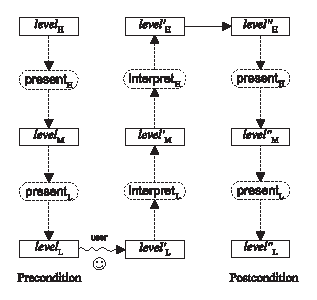
\epsfig{file=pics/eps/LayerCombined.eps, height=2in} % visio: Layer.vsd
\end{center}\caption{Single edit step in a composite layer.} \label{compositeEdit}
\end{center}
\end{small}
\end{figure}

%\begin{figure}
%\xpr{
%level\H 		&   			& level'\H 	&~\rightarrow~& level''\H\\
%~~~\downarrow&   		&~~~\uparrow&			&~~~\downarrow \\
%level\M 		&   			& level'\M 	& 			& level''\M\\
%~~~\downarrow 	&   		&~~~\uparrow&			&~~~\downarrow \\
%level\L 		&~\leadsto~& level'\L 	& 			& level''\L\\
%} \caption{Single edit step in a composite layer. (draft)} \label{compositeEdit}
%\end{figure}

Before the lower level is updated, we have:

\xpr{
\eqcl{\level\L}{LL} = \present\L~\eqcl{\level\M}{LH} ~\land~
\eqcl{\level\M}{HL} = \present\H~\eqcl{\level\H}{HH}\\
\level\L \leadsto \level'\L 
}

After the lower-level update, the lower layer computes an intermediate value $\level'\M$, from which the higher layer (which may be a composite layer itself) computes $\level'\H$. At the top, $\level'\H$ is assigned to $\level''\H$, which is subsequently presented onto $level''\M$. Finally, $level''\M$ presented onto $level''\L$. 

Figure~\ref{compositeEdit} sketches the updates to the various data levels. Note that the figure is just a sketch, since $\present$ and $\interpret$ are functions between equivalence classes instead of values (as the figure might suggest). 

\head{Requirements}

Apart from a few changes to the subscripts, the requirements for $level''\H$ and $level''\L$ are equal to the requirements for the single-layered editor in Section~\ref{sect:singleExtra_Editing}. The only difference is that we explicitly added the precondition of the edit step ($\eqcl{\level\L}{CL} = \present\C~\eqcl{\level\H}{CH}$) to the precondition of \law{Doc-Inert}. We need it here, because \law{Doc-Inert} can only hold if the middle level is a valid presentation of $\level\H$. 

\xprlab{\hoare{\true} {Comp} { \eqcl{\level''\L}{CL} = \present\C~\eqcl{\level''\H}{CH} } }		{Postcondition}
%\xprlab{\hoare{\eqcl{\level\L}{L} = \present\C~\eqcl{\level\H}{H} \land \eqcl{\level'\L}{CL} = %\present\C~\eqcl{\level\H}{CH}} {Comp} { \level\H = \level''\H}}  {Doc-Inert}
\xprlab{ 
\left\{ \begin{array}{l}
 \eqcl{\level\L}{CL} = \present\C~\eqcl{\level\H}{CH} ~\land\\
 \eqcl{\level'\L}{CL} = \present\C~\eqcl{\level\H}{CH}
\end{array}\right\}
{Comp} \{ \level\H = \level''\H\} }  {Doc-Inert}
\xprlab{\hoare{\eqcl{\level'\L}{CL} = \present\C~\eqcl{h}{CH}} {Comp} { \level'\L = \level''\L}}		{Pres-Inert}
\xprlab{\hoare{\true} {Comp} {\level\H \close \level''\H}}	{Doc-Preserve}
\xprlab{\hoare{\true} {Comp} {\level'\L \close \level''\L}}	{Intended}

\head{Definition of $Comp$}

The inductive definition of $Comp$ reads:

\xprlab{
Comp_0 \is 	& \level''\H \gets \level'\H\\
Comp_n \is 	& Up \semi Comp_{n-1} \semi Dwn}{$Comp$-Def}
\xprlab{
Up \is		& \level'\M \gets \interpret\L~ \eqcl{\level'\L}{LL}  ~\reuze{LH}~   \level\M}{$Up$-Def}
\xprlab{
Dwn \is		& \level''\L \gets \present\L~ \eqcl{\level''\M}{LH}   ~\reuze{LL}~   \level'\L}{$Dwn$-Def}

We prove that $Comp$ meets the first three requirements.


\subsection{\law{Postcondition} requirement}

In \fn{wp} notation, the \law{Postcondition} is:

\xprlab{\true ~~\imp~~ \wp{Comp_n}{\eqcl{\level''\L}{CL} = \present\C~\eqcl{\level''\H}{CH}}} {Postcondition}


\begin{proof} We prove \law{Postcondition} by induction over the number of layers $n$. 

{\bf Case} $n=0$:

Filling in the base cases for $present\C$, the data levels, and relations $CH$ and $CL$ yields:

\xpr{\true ~~\imp~~ \wp{Comp}{\eqcl{\level''_0}{=} = \id~\eqcl{\level''_0}{=}}}

which holds because it is equivalent to $\true ~\imp~ \wp{Comp}{\true}$.

{\bf Case} $n>0$:

%\eqcl{l}{CL} = \present\C~\eqcl{h}{CH} & ~\eqv~ & \exists m :~
%			& \eqcl{l}{LL}	& = \present\L~\eqcl{m}{LH}\\
% & &~~\land	& \eqcl{m}{HL}	& = \present\H~\eqcl{h}{HH}
The induction hypothesis is:

\xprlab{\true ~~\imp~~ \wp{Comp_{n-1}}{ \eqcl{\level''\M}{HL} = \present\H~\eqcl{\level''\H}{HH}}} {I.H.}

In the proof, we need the property that the lower presentation of a valid middle level is in the result of the composite presentation:

\xpr{
\eqcl{m}{HL} = \present\H~\eqcl{h}{HH} ~~\imp~~ \eqcl{\present\L~ \eqcl{m}{LH}   ~\reuze{LL}~   l}{CL} = \present\C~\eqcl{h}{CH} \\
}

It has a simple proof:

\begin{Prf}&
	\eqcl{\present\L~ \eqcl{m}{LH}   ~\reuze{LL}~   l}{CL} = \present\C~\eqcl{h}{CH} \\
\Eqv{\law{$\present$-Compose}}&
 	\exists m' :\eqcl{\present\L~ \eqcl{m}{LH}   ~\reuze{LL}~   l}{LL} = \present\L~\eqcl{m'}{LH} \land
 	\eqcl{m'}{HL} = \present\H~\eqcl{h}{HH}\\
\Ffr{let $m' = m$}&
 	\eqcl{\present\L~ \eqcl{m}{LH}   ~\reuze{LL}~   l}{LL} = \present\L~\eqcl{m}{LH} \land
 	\eqcl{m}{HL} = \present\H~\eqcl{h}{HH}\\
\Eqv{\law{$\reuz$-Valid}}&
 	\present\L~ \eqcl{m}{LH} = \present\L~\eqcl{m}{LH} \land
 	\eqcl{m}{HL} = \present\H~\eqcl{h}{HH}\\
\Eqv{reflexivity of $=$}&
	\eqcl{m}{HL} = \present\H~\eqcl{h}{HH} \\
\end{Prf}


Using this result, we prove \law{Postcondition}.

\begin{Prf}&
	\wp{Comp}{\eqcl{\level''\L}{CL} = \present\C~\eqcl{\level''\H}{CH}}\\
\Eqv{\law{$Comp$-Def}}&
	\wp{Up \semi Comp_{n-1} \semi Dwn}{ \eqcl{\level''\L}{CL} = \present\C~\eqcl{\level''\H}{CH} }\\
\Eqv{\law{\fn{wp}-$\smi$}}&
	\wp{Up \semi Comp_{n-1}}{ \wp{Dwn }{ \eqcl{\level''\L}{CL} = \present\C~\eqcl{\level''\H}{CH} }}\\
\Eqv{\law{$Dwn$-Def}}&
	\fn{wp}({Up \semi Comp_{n-1}},~{ \wpWide{\level''\L \gets \present\L~ \eqcl{\level''\M}{LH}   ~\reuze{LL}~   \level'\L}{ \eqcl{\level''\L}{CL} = \present\C~\eqcl{\level''\H}{CH} )} }  \\
\Eqv{\law{\fn{wp}-$\gts$}}&
	\wp{Up \semi Comp_{n-1}}{ \eqcl{\present\L~ \eqcl{\level''\M}{LH}   ~\reuze{LL}~   \level'\L}{CL} = \present\C~\eqcl{\level''\H}{CH} }\\
\Ffr{\law{\fn{wp}-Mono} and previous result}&
	\wp{Up \semi Comp_{n-1}}{\eqcl{\level''\M}{HL} = \present\H~\eqcl{\level''\H}{HH}} \\
\Eqv{\law{\fn{wp}-$\smi$}}&
	\wp{Up}{ \wp{ Comp_{n-1}}{  \eqcl{\level''\M}{HL} = \present\H~\eqcl{\level''\H}{HH} }}\\
\Ffr{\law{\fn{wp}-Mono} and \law{I.H.}}&
	\wp{Up}{ \true}\\
\Eqv{\law{$Up$-Def}}&
	\wp{\level'\M \gets \interpret\L~ \eqcl{\level'\L}{LL}  ~\reuze{LH}~   \level\M}{ \true }\\
\Eqv{\law{\fn{wp}-$\gts$}}&
	\true\\
\end{Prf}
\end{proof}






\subsection{\law{Doc-Inert} requirement}

\xprlab{\eqcl{\level\L}{CL} = \present\C~\eqcl{\level\H}{CH} \land \eqcl{\level'\L}{CL} = \present\C~\eqcl{\level\H}{CH} ~~\imp\\ \wp{Comp_n}{\level\H = \level''\H}}{\hspace{-2em}Doc-Inert}
 
Besides the {$\present$-Match} and {$\interpret$-Match} conditions from Section~\ref{sect:compositeExtraCompose}, we need an additional condition for \law{Doc-Inert} to hold. From \law{InterPresent}, we know that if $\level'\L$ is a presentation of $\level\H$, then $\level\H$ is in the interpretation of $\level'\L$. Thus, there exists a middle level $m$ in the interpretation of $\level'\L$, which has $\level\H$ in its interpretation. However, the mere existence of such a middle level does not guarantee that this is the middle level resulting from $Comp$.

The problem lies in the fact that $level'\M$ is selected by $\reuze{LH}$ from an $LH$ class of elements, instead of an $HL$ class. Thus, reusing extra state from $level\M$ could cause $\level'\M$ to end up in an $HL$ class that does not contain $level\M$, which would break \law{Doc-Inert}. We avoid the problem by requiring that the result of $\reuze{LH}$ is in the correct $HL$ class, if possible:

\xprlab{
\eqcl{m'}{HL} = \eqcl{m}{HL} ~\imp~ \eqcl{\eqcl{m'}{LH} \reuze{LH} m}{HL} = \eqcl{m}{HL}}{Orthogonal}

If both $HL$ and $LH$ are described by the wildcard types from Section~\ref{sect:wildcardEq}, \law{Orthogonal} holds.
%\note{prove this?}


%
%\xprlab{
%\eqcl{m'}{HL} = \eqcl{m}{HL} ~\imp~ \eqcl{m'}{LH} \reuze{LH} m \in \eqcl{m}{HL}}{Orthogonal}
%
%
%Different notation:
%\xprlab{
%m'~HL~m ~\imp~ \eqcl{m'}{LH} \reuze{LH} m~HL~m}{Orthogonal}


%\xprlab{\hoare{\eqcl{\level'\M}{HL} = \present\H~\eqcl{\level\H}{H}} {Comp_{n-1}} { \level\H = \level''\H}}{I.H.}

\begin{proof}

The proof of \law{Doc-Inert} is by induction over $n$. 

{\bf Case} $n=0$:

\xpr{\eqcl{\level_0}{=} = \id~\eqcl{\level_0}{=} \land \eqcl{\level'_0}{=} = \id~\eqcl{\level_0}{=} ~\imp~ \wp{Comp_0}{\level_0 = \level''_0}}

%\xpr{\true ~\imp~ \wp{Comp}{\eqcl{\level''_0}{=} = \id~\eqcl{\level''_0}{=}}}

\begin{Prf}&
	\wp{Comp_0}{\level_0 = \level''_0}\\
\Eqv{\law{$Comp$-Def} and $\Level\H \eqv \Level_0$}&
	\wp{\level''_0 \gets \level'_0}{\level_0 = \level''_0}\\
\Eqv{\law{\fn{wp}-$\gts$}}&
	\level_0 = \level'_0\\
\Ffr{property of equivalence class and symmetry of $=$}&
	\level'_0 \in \eqcl{\level_0}{=}\\
\Ffr{\law{$\eqhole$-Member}}&
	\eqcl{\level_0}{=} = \eqcl{\level_0}{=} \land \eqcl{\level'_0}{=} = \eqcl{\level_0}{=}\\
\Eqv{definition of $\id$}&
	\eqcl{\level_0}{=} = \id~\eqcl{\level_0}{=} \land \eqcl{\level'_0}{=} = \id~\eqcl{\level_0}{=}\\
\end{Prf}


{\bf Case} $n>0$:

For the inductive case, we assume the antecedent of the implication. The first conjunct 
($\eqcl{\level\L}{CL} = \present\C~\eqcl{\level\H}{CH}$) has already been rewritten according to \law{$\present$-Compose} and the implicit assumption that the middle level between $level\H$ and $\level\L$ is $level\M$:

\xpr{\eqcl{\level\L}{LL} = \present\L~\eqcl{\level\M}{LH} ~\land~ \eqcl{\level\M}{HL} = \present\H~\eqcl{\level\H}{HH} ~\land~\\
 \eqcl{\level'\L}{L} = \present\C~\eqcl{\level\H}{H}}


In the proof, we need the existence of an $m_0$ that is in the equivalence class of the interpretation of $\level'\L$ and at the same time in the equivalence class of the presentation of $\level\H$:

\begin{Prf}&
	\eqcl{m_0}{LH} = \interpret\L~\eqcl{\level'\L}{LL} ~\land~ \eqcl{m_0}{HL} = \present\H~\eqcl{\level\H}{HH}\\
\FFr{let $m_0$ be the $m$ from the quantification}&
	\exists m : \eqcl{m}{LH} = \interpret\L~\eqcl{level'\L}{LL} ~\land~ \eqcl{m}{HL} = \present\H~\eqcl{\level\H}{HH}\\
\Eqv{\law{InterPresent}}&
	\exists m : \eqcl{level'\L}{LL} = \present\L~\eqcl{m}{LH} ~\land~ \eqcl{m}{HL} = \present\H~\eqcl{\level\H}{HH}\\
\Eqv{\law{$\present$-Compose}}&
	\eqcl{level'\L}{CL} = \present\C~\eqcl{\level\H}{CH}\\
\Eqv{assumption}&
	\true\\
\end{Prf}
          
%\begin{Prf}&
%	\eqcl{m_0}{HL}\\
%\Equ{$\eqcl{m_0}{HL} = \present\H~\eqcl{\level\H}{HH}$}&
%	\present\H~\eqcl{\level\H}{HH}\\
%\Equ{\law{Present}}&
%	\eqcl{\level\M}{HL}\\
%\end{Prf}

Together with $\present\H~\eqcl{\level\H}{HH} = \eqcl{\level\M}{HL}$ from the precondition,
$\eqcl{m_0}{HL} = \present\H~\eqcl{\level\H}{HH}$ implies that $m_0$ and $\level\M$ are in the same $HL$ class: $\eqcl{m_0}{HL}=\eqcl{\level\M}{HL}$. This result is needed in order to apply \law{Orthogonal}.

% can be put in linear wp proof
%\begin{Prf}&
%	\eqcl{\interpret\L~ \eqcl{\level'\L}{LL}  ~\reuze{LH}~   \level\M}{HL}\\
%\Equ{$\eqcl{m_0}{LH} = \interpret\L~\eqcl{\level'\L}{LL}$}&
%	\eqcl{\eqcl{m_0}{LH}   ~\reuze{LH}~   \level\M}{HL}\\
%\Equ{\law{Orthogonal} (different notation) + $\eqcl{m_0}{HL}=\eqcl{\level\M}{HL}$}&
%	\eqcl{m_0}{HL}\\
%\Equ{\law{$\eqcl{m_0}{HL} = \present\H~\eqcl{\level\H}{HH}$}}&
%	\present\H~\eqcl{\level\H}{HH}\\
%\end{Prf}


For the inductive step, we have the following induction hypothesis:

\xprlab{\eqcl{\level\M}{HL} = \present\H~\eqcl{\level\H}{HH} ~\land~ \eqcl{\level'\M}{HL} = \present\H~\eqcl{\level\H}{HH} ~~\imp\\ \wp{Comp_{n-1}}{\level\H = \level''\H}}{I.H.}

Note that the first conjunct in the antecedent of the induction hypothesis is already satisfied due to the assumption above.

Because we assumed the antecedent of \law{Doc-Inert} (in weakest precondition notation), we complete the proof of the implication by proving its conclusion.

\begin{Prf}&
	\wp{Comp_n}{\level\H = \level''\H}\\
\Eqv{\law{$Comp$-Def}}&
	\wp{Up \semi Comp_{n-1} \semi Dwn}{ \level\H = \level''\H }\\
\Eqv{\law{\fn{wp}-$\smi$}}&
	\wp{Up \semi Comp_{n-1}}{ \wp{Dwn }{ \level\H = \level''\H }}\\
\Eqv{\law{$Dwn$-Def}}&
	\wpWide{Up \semi Comp_{n-1}}{ \wp{\level''\L \gets \present\L~ \eqcl{\level''\M}{LH}   ~\reuze{LL}~   \level'\L}{ \level\H = \level''\H }}\\
\Eqv{\law{\fn{wp}-$\gts$}}&
	\wp{Up \semi Comp_{n-1}}{ \level\H = \level''\H }\\
\Eqv{\law{\fn{wp}-$\smi$}}&
	\wp{Up}{ \wp{ Comp_{n-1}}{ \level\H = \level''\H }}\\
\Ffr{\law{\fn{wp}-Mono}, \law{I.H.}, and $\eqcl{\level\M}{HL} = \present\H~\eqcl{\level\H}{HH}$}&
	\wp{Up}{ \eqcl{\level'\M}{HL} = \present\H~\eqcl{\level\H}{HH}}\\
\Eqv{\law{$Up$-Def}}&
	\wpWide{\level'\M \gets \interpret\L~ \eqcl{\level'\L}{LL}  ~\reuze{LH}~   \level\M}{ \eqcl{\level'\M}{HL} = \present\H~\eqcl{\level\H}{HH} }\\
\Eqv{\law{\fn{wp}-$\gts$}}&
%	\eqcl{\interpret\L~ \eqcl{\level'\L}{LL}  ~\reuze{LH}~   \level\M}{HL} =  \present\H~\eqcl{\level\H}{HH}\\
%\end{Prf}  
%\begin{Prf}& 
	\eqcl{\interpret\L~ \eqcl{\level'\L}{LL}  ~\reuze{LH}~   \level\M}{HL} = \present\H~\eqcl{\level\H}{HH}\\
\Eqv{$\eqcl{m_0}{LH} = \interpret\L~\eqcl{\level'\L}{LL}$}&
	\eqcl{\eqcl{m_0}{LH}   ~\reuze{LH}~   \level\M}{HL} = \present\H~\eqcl{\level\H}{HH}\\
\Eqv{\law{Orthogonal} and $\eqcl{m_0}{HL}=\eqcl{\level\M}{HL}$}&
	\eqcl{m_0}{HL} = \present\H~\eqcl{\level\H}{HH}\\
\Eqv{\law{$\eqcl{m_0}{HL} = \present\H~\eqcl{\level\H}{HH}$}}&
	\present\H~\eqcl{\level\H}{HH} = \present\H~\eqcl{\level\H}{HH}\\
\Eqv{symmetry of $=$}&
	\true\\
\end{Prf}
\end{proof}





\subsection{\law{Pres-Inert} requirement}

\xprlab{\eqcl{\level'\L}{CL} = \present\C~\eqcl{h}{CH} ~~\imp~~ \wp{Comp_n} { \level'\L = \level''\L}}		{Pres-Inert}

Similar to \law{Doc-Inert}, we cannot guarantee \law{Pres-Inert} without assuming extra conditions. It turns out that we can prove \law{Pres-Inert} if we assume \law{$\present$-Match} \nonote{not \law{$\interpret$-Match}??} together with a reversed \law{Orthogonal}, in which the $HL$ and $LH$ relations are swapped. However, because \law{Orthogonal} refers to $\reuze{LH}$, its reverse would have to refer to $\reuze{HL}$, which does not exist. The reason for this is the association order in $Comp$: reuse in the presentation direction of the higher layer is the result of the combined effect of the $\reuze{LL}$ functions of the components of the higher layer. Thus, the only way to specify a reversed \law{Orthogonal} is as a condition on the composite layer:

\xprlab{
\eqcl{\level'\L}{LH}  = \eqcl{m}{LH} ~\imp~ \wp{Comp_{n-1}} {\eqcl{\level''\L}{LH}  = \eqcl{m}{LH}}}{Orthogonal-R}

Because this condition is rather complex, we introduce a stronger condition \law{Absorption} that is easier to verify. \law{Absorption} implies \law{$\present$-Match} and \law{$\interpret$-Match}, as well as \law{Orthogonal} and \law{Orthogonal-R}.

%
%PROBLEM:
%\xprlab{
%\eqcl{m'}{LH} = \eqcl{m}{LH} ~\imp~ \eqcl{\eqcl{m'}{HL} \reuze{HL} m}{LH} = \eqcl{m}{LH}}{Orthogonal-R}
%
%There is no $\reuze{HL}$, because it is the composition of several $\reuze{LL}$'s in the higher layers. This definition is %therefore not valid. 
%
%Furthermore, \law{Absorption} as defined below 
%
%There seem to be two options.
%
%1) No to mention \law{Orthogonal-R} at all and always assume \law{Absorption}. A separate 
%
%2) Introduce this definition of \law{Orthogonal-R}:
%
%\xprlab{
%\eqcl{\level'\L}{LH}  = \eqcl{m}{LH} ~\imp~ \wp{Comp_{n-1}} {\eqcl{\level''\L}{LH}  = \eqcl{m}{LH}}}{Orthogonal-R}
%
%
%For $Layer_1$ (composition of ($\present_1$,$interpret_1$) with ($\id$,$\id$)), we can easily prove that \law{Orthogonal-R} %always holds. 
%
%For the rest of the layers, we assume \law{Absorption}
%
%

%However, because the precondition of \law{Pres-Inert} does not guarantee that the intermediate level is valid, we cannot use %\law{Pres-Inert} inductively on the higher layer. As a consequence, the proof of \law{Pres-Inert} becomes very tedious. 

%In order to simplify the proof, we introduce a stronger condition \law{Absorption}, which can be proven to imply both %\law{$\present$-Match} and \law{$\interpret$-Match}, as well as \law{Orthogonal}. 

%\xprlab{
%\forall m : \eqcl{m}{LH} \subset \eqcl{m}{HL}}{Absorption}

\xprlab{
\eqcl{m}{LH} = \eqcl{m'}{LH} ~\imp~ \eqcl{m}{HL} = \eqcl{m'}{HL}}{Absorption}

The condition states that two $Level\M$ values that are in the same $LH$ equivalence class of the lower layer, also share the $HL$ equivalence class of the higher layer. Thus, interpretation extra state on the middle level is absorbed by presentation extra state on that level, hence the name.

As an example of \law{Absorption} for the wildcard types of Section~\ref{sect:wildcardEq}, consider the $LH$ relation represented by $(Int,(Int,*_{Int}))$.  This relation is absorbed by an $HL$ relation $(Int,(*_{Int},*_{Int}))$, and also by $(Int,*_{Int})$. 

For wildcard types, \law{Absorption} holds if and only if for all possible values of type $Level\M$, any node that is a $\texttt{*}$ according to the wildcard definition of $LH$, is either also a $\texttt{*}$ according to $HL$ or has an ancestor that is a $\texttt{*}$.

More generally, \law{Absorption} holds when each $HL$ equivalence class is a union of $LH$ classes. A result of \law{Absorption} is that  $CH$ is equal to $HH$. For the proof of \law{Pres-Inert}, \law{Absorption} implies that the intermediate level that results from interpreting a valid lower level, is itself also valid, which allows us to apply \law{Pres-Inert} inductively to the higher layer.


\bc We do not wish to assume \law{Absorption} for the top-most composition ($\present_1$, $\interpret_1$ and the identity), because it implies that the interpretation extra state of $\present_1$ is absorbed by the presentation extra state of $\id$. As a consequence, the top-most composition would not have interpretation extra state. Furthermore, due to absorption, each composite equivalence relation $CH_i$ is equal to $HH$ (or $CH_{i-1}$), 
\ec

Because of \law{Absorption} we have  $CH = HH$. If we denote this with the explicit indices from Figure~\ref{indicesInLayer}, we get $CH_i = CH_{i-1}$. Furthermore, since $CH_0 ~=~ (=)$, this means that $CH_i~=~(=)$, and, thus, no composite layer has interpretation extra state on $Level_0$. This is clearly not a desirable situation, and hence we do not assume \law{Absorption} for the top-most combination. Nevertheless, the result is still quite restrictive, since now the interpretation extra state relation $CH_i$ for each composite layer will be equal to the interpretation extra state relation $H_1$ for $\present_1$. Future research should determine whether this is a problem. If it is, a less-strict condition will need to be established.

Because we do not assume \law{Absorption} at the top-most composite layer, we have to give a separate proof for case $n=1$ of \law{Pres-Inert}, in which we do not use the condition. Furthermore, in the proof of \law{Doc-Inert}, we cannot use \law{Absorption} to imply \law{$\present$-Match}, \law{$\interpret$-Match}, and \law{Orthogonal} for case $n=1$. However, since for $n=1$, these three conditions trivially hold, we do not need to assume \law{Absorption} for this case.


\begin{proof}
In the inductive step of the proof, we need the fact that the lower level is not affected by the assignments of the higher layer. Therefore, we strengthen the pre- and postcondition of \law{Pres-Inert}:

\xpr{ \eqcl{\level'\L}{CL} = \present\C~\eqcl{h}{CH}  ~\land~ \level'_{n+1} = x ~~\imp\\ \wp{Comp_n}{\level'\L = \level''\L  ~\land~ \level'_{n+1} = x}}

%Here we need:
%
%which implies
%
%\begin{Prf}&
%	\eqcl{\level'\L}{CL} = \present\C~\eqcl{h}{CH}\\
%\Imp{magic}&
%	\eqcl{\level'\L}{CL} = \present\C~\eqcl{h}{CH} \land \level_{n+1} = x\\
%\Imp{assumption}&
%	\wp{Comp_n}{\level'\L = \level''\L  \land \level_{n+1} = x}\\
%\Imp{\law{\fn{wp}-Mono} and $X \land Y ~\imp~ X$}&
%	\wp{Comp_n}{\level'\L = \level''\L}\\
%\end{Prf}

\bc
{\bf Case} $n=0$:

The base case

\xpr{\eqcl{\level'_0}{=} = \id~\eqcl{h}{=} \land \level'_{1} = x ~\imp~\wp {Comp_0} { \level'_0 = \level''_0 \land \level'_{1} = x}}

is evident if we substitute according to \law{$Comp$-Def}:

\xpr{\eqcl{\level'_0}{=} = \id~\eqcl{h}{H} \land \level'_{1} = x ~\imp~\wp {\level''_0 \gets \level'_0} { \level'_0 = \level''_0 \land \level'_{n+1} = x}}
\ec

{\bf Case} $n=0$: We omit the trivial proof of this case. 
%mention we don't need it because we give $n=1$? (and since $n=0$ is only for \id-layer)

{\bf Case} $n=1$:

%\xpr{ \eqcl{\level'\L}{CL} = \present\C~\eqcl{h}{CH}  \land \level'_{n+1} = x ~\imp\\ \wp{Comp_n}{\level'\L = \level''\L  \land %\level'_{n+1} = x}}
For $n=1$,  we have $level\H = level\M = level_0$ and $level\L = level_1$. Furthermore, since 
$present\H = \present_{\mathrm{C},0} = \id$ and $HH$ and $HL$ both are $(=)$, we have $\present\C~\eqcl{h}{CH} = \present\L~\eqcl{h}{LH}$. Thus, we rewrite the requirement to: 
 
\xpr{ \eqcl{\level'\L}{LH} = \present\L~\eqcl{h}{LH}  ~\land~ \level'_{2} = x ~~\imp\\ \wp{Comp_1}{\level'\L = \level''\L  ~\land~ \level'_{2} = x}}


First, we prove the first conjunct of the postcondition, for which we only need to assume half of the antecedent 
$\eqcl{\level'\L}{LL} = \present~\eqcl{h}{LH}$. The proof is similar to the proof of \law{Pres-Inert} for a single layer (see Section~\ref{sect:singleExtra_Editing}).

	
\begin{Prf}&
	\wp{Comp_1}{ \level'\L = \level''\L  }\\
\Eqv{\law{$Comp$-Def}}&
	\wp{Up \semi Comp_0 \semi Dwn}{ \level'\L = \level''\L  }\\
\Eqv{\law{\fn{wp}-$\smi$}}&
	\wp{Up \semi Comp_0}{\wp{Dwn}{ \level'\L = \level''\L  }}\\
\Eqv{\law{$Dwn$-Def}}&
	\wp{Up \semi Comp_0}{\wp{\level''\L \gets \present~ \eqcl{\level''\M}{LH}   ~\reuze{LL}~   \level'\L}{ \level'\L = \level''\L  }}\\
\Eqv{\law{\fn{wp}-$\gts$}}&
	\wp{Up \semi Comp_0}{\level'\L = \present~ \eqcl{\level''\M}{LH}   ~\reuze{LL}~   \level'\L }\\
\Eqv{\law{\fn{wp}-$\smi$}}&
	\wp{Up}{\wp{Comp_0}{\level'\L = \present~ \eqcl{\level''\M}{LH}   ~\reuze{LL}~   \level'\L }}\\
\Eqv{\law{$Comp$-Def} and $Level\M \eqv \Level_0$}&
	\wp{Up}{\wp{\level''\M \gets \level'\M}{\level'\L = \present~ \eqcl{\level''\M}{LH}   ~\reuze{LL}~   \level'\L }}\\
\Eqv{\law{\fn{wp}-$\gts$}}&
	\wp{Up}{\level'\L = \present~ \eqcl{\level'\M}{LH}   ~\reuze{LL}~   \level'\L }\\
\Eqv{\law{$Up$-Def}}&
	\wpWide{\level'\M \gets \interpret~ \eqcl{\level'\L}{LL}  ~\reuze{LH}~   \level\M}{\level'\L = \present~ \eqcl{\level'\M}{LH}   ~\reuze{LL}~   \level'\L }\\
\Eqv{\law{\fn{wp}-$\gts$}}&
	\level'\L = \present~ \eqcl{\interpret~ \eqcl{\level'\L}{LL}  ~\reuze{LH}~   \level\M}{LH}   ~\reuze{LL}~   \level'\L\\
\Eqv{assumption}&
	\level'\L = \present~ \eqcl{\interpret~(\present~\eqcl{h}{LH})  ~\reuze{LH}~  \level\M}{LH}   ~\reuze{LL}~   \level'\L\\
\Eqv{\law{InterPresent }}&
	\level'\L  = \present~ \eqcl{\eqcl{h}{LH}  ~\reuze{LH}~   \level\M}{LH}   ~\reuze{LL}~   \level'\L\\
\Eqv{\law{$\reuz$-Valid}}&
	\level'\L  = \present~\eqcl{h}{LH}  ~\reuze{LL}~  \level'\L\\
\Eqv{assumption}&
	\level'\L  = \eqcl{\level'\L}{LL}~\reuze{LL}~  \level'\L\\
\Eqv{\law{$\reuz$-Idem} }&
	\eqcl{\level'\L}{LL} = \eqcl{\level'\L}{LL}\\
\Eqv{reflexivity of $=$}&
	\true\\
\end{Prf}

This completes the proof of the first conjunct of the postcondition. For the second conjunct, we need to prove:

\xpr{ \eqcl{\level'\L}{LH} = \present\L~\eqcl{h}{LH}  ~\land~ \level'_{2} = x ~~\imp\\ \wp{Comp_1}{\level'_{2} = x}}

which trivially holds, because $Comp_1$ only performs assignments on levels~0 and~1. Hence, by \law{\fn{wp}-And}, we conclude: 

\xpr{ \eqcl{\level'\L}{LH} = \present\L~\eqcl{h}{LH}  ~\land~ \level'_{2} = x ~~\imp\\ \wp{Comp_1}{\level'\L = \level''\L  ~\land~ \level'_{2} = x}}

%\xpr{\hoare{\eqcl{\level'\L}{L} = \present~\eqcl{h}{H}} {Comp_n} { \level'\L = \level''\L}}


%\xpr{ \eqcl{\level'_0}{H} = \present_0~\eqcl{h}{H} ~\imp~ \wp{Comp_0}{\level'_0 = \level''_0}} 
%
%\begin{Prf}
%\Eqv{\law{\fn{wp}-$\gts$}}&
%	\wp{\level''\H \gets \interpret\L~\level'\L}{ \wp{ \level''\L \gets \present~\level''\H}{\level\H = \level''\H}} \\
%\Eqv{\law{\fn{wp}-$\smi$}}&
%	\wp{\level''_0 \gets \level'_0}{\level_0 = \level''\H} \\
%\Eqv{\law{$Comp$-Def}}&
%	\wp{Comp_0}{\level'_0 = \level''_0}\\
%\end{Prf}

{\bf Case} $n>1$:

Similar to the $n=1$ case, prove the first part of postcondition conjunct:

\xpr{ \eqcl{\level'\L}{CL} = \present\C~\eqcl{h}{CH} ~\land~ \level'_{n+1} = x  ~~\imp~~ \wp{Comp_n}{\level'\L = \level''\L}}

We assume half of the antecedent: $\eqcl{\level'\L}{CL} = \present\C~\eqcl{h}{CH}$.


%result of $Up$ and $m_0$ are in same LH class.
%
%does not seem to work:
%\begin{Prf}&
%	(\interpret\L~ \eqcl{\level'\L}{LL})  \reuze{LH}   \level\M  \\
%\Eqv{$\eqcl{m_0}{LH} = \interpret\L~\eqcl{level'\L}{LL}$}&
%	\eqcl{m_0}{LH}  \reuze{LH}   \level\M  \\
%\Imp{\law{$\reuz$-Valid}}&
%	\eqcl{m_0}{LH}\\
%\Imp{\law{Absorption}}&
%	\level'\M \in \eqcl{m_0}{HL}\\
%\Imp{\law{$\eqhole$-Member}}&
%	\eqcl{\level'\M}{HL} = \eqcl{m_0}{HL}\\
%\end{Prf}
%\note{rewrite valid? or just mention that it can be rewritten (as = on eq. classes)}
%\xpr{
%\eqcl{\interpret\L~ \eqcl{\level'\L}{L}  ~\reuze{H}~  \level\M}{HL} = \present\H~\eqcl{h}{HH} \\
%}


From the assumption, we know there exists an $m_0$ that is in the presentation of $h$, and that has $\level'\L$ in its presentation:

\begin{Prf}&
	\eqcl{level'\L}{LL} = \present\L~\eqcl{m_0}{LH} ~\land~ \eqcl{m_0}{HL} = \present\H~\eqcl{h}{HH}\\
\Eqv{let $m_0$ be the $m$ from the quantification}&
	\exists m : \eqcl{level'\L}{LL} = \present\L~\eqcl{m}{LH} ~\land~ \eqcl{m}{HL} = \present\H~\eqcl{h}{HH}\\
\Eqv{\law{$\present$-Compose}}&
	\eqcl{level'\L}{CL} = \present\C~\eqcl{h}{CH}\\
\Eqv{assumption}&
	\true\\
\end{Prf}

Furthermore, by the first part of this conjunct and \law{InterPresent} on the lower layer, we also have $\eqcl{m_0}{LH} = \interpret\L~\eqcl{level'\L}{LL}$
%$\eqcl{m_0}{HL} = \present\H~\eqcl{h}{HH}$


%Define an $m'$ to be $(\interpret\L~ \eqcl{\level'\L}{LL})  \reuze{LH}   \level\M$
%\begin{Prf}&
%	\true\\
%\Eqv{ bla }&
%	m' = (\interpret\L~ \eqcl{\level'\L}{LL})  \reuze{LH}   \level\M  \\
%\Imp{$\eqcl{m_0}{LH} = \interpret\L~\eqcl{level'\L}{LL}$}&
%	m' = \eqcl{m_0}{LH}  \reuze{LH}   \level\M  \\
%\Imp{\law{$\reuz$-Valid}}&
%	m' \in \eqcl{m_0}{LH}\\
%\Imp{\law{Absorption}}&
%	m' \in \eqcl{m_0}{HL}\\
%\Imp{\law{$\eqhole$-Member}}&
%	\eqcl{m'}{HL} = \eqcl{m_0}{HL}\\
%\Eqv{\law{$\eqhole$-Member}}&
%	\eqcl{(\interpret\L~ \eqcl{\level'\L}{LL})  \reuze{LH}   \level\M}{HL} = \eqcl{m_0}{HL}\\
%\end{Prf}

%or alternatively: using rewritten \law{Absorption}
%\eqcl{m}{LH} = \eqcl{m'}{LH} ~\imp~ \eqcl{m}{HL} = \eqcl{m'}{HL}}{Absorption}
We need two intermediate results for the inductive step of the proof. The first one is:

% states that the intermediate valua after interpret of lower layer is in presentation of $h$, hence precondition for doc-inert on higher layer is satis.

\begin{Prf}&
	\eqcl{\interpret\L~ \eqcl{\level'\L}{LL}  ~\reuze{LH}~  \level\M}{HL} = \present\H~\eqcl{h}{HH} \\
\Equ{$\eqcl{m_0}{HL} = \present\H~\eqcl{h}{HH}$}&
	\eqcl{\interpret\L~ \eqcl{\level'\L}{LL}  \reuze{LH}   \level\M}{HL} = \eqcl{m_0}{HL}\\
\Ffr{\law{Absorption}}&
	\eqcl{\interpret\L~ \eqcl{\level'\L}{LL}  \reuze{LH}   \level\M}{LH} = \eqcl{m_0}{LH}\\
\Eqv{$\eqcl{m_0}{LH} = \interpret\L~\eqcl{level'\L}{LL}$}&
	\eqcl{\eqcl{m_0}{LH}  \reuze{LH}   \level\M}{LH} = \eqcl{m_0}{LH}\\
\Eqv{\law{$\reuz$-Valid}}&
	\eqcl{m_0}{LH} = \eqcl{m_0}{LH}\\
\Eqv{reflexivity of $=$}&
	\true\\
\end{Prf}

A corollary of this proof is that $\eqcl{\interpret\L~ \eqcl{\level'\L}{LL}  ~\reuze{LH}~   \level\M}{LH} = \eqcl{m_0}{LH}$, which is used in the proof of the second intermediate result:

% which states that if the middle (same as intermediate due to doc-inert) is presented, we get level'L again.


% this used to be a separate proof
%For the first equality in conjunct:
%\xpr{
%\eqcl{\interpret\L~ \eqcl{\level'\L}{L}  ~\reuze{LH}~  \level\M}{HL} = \present\H~\eqcl{h}{HH} \\
%}
%
%\begin{Prf}&
%	\eqcl{(\interpret\L~ \eqcl{\level'\L}{LL})  \reuze{LH}   \level\M}{HL}\\
%\Equ{previous result}&
%	\eqcl{m_0}{HL}\\
%\Equ{$\eqcl{m_0}{HL} = \present\H~\eqcl{h}{HH}$}&
%	\present\H~\eqcl{h}{HH}\\
%\end{Prf}


\xpr{
\level'\L = \present\L~ \eqcl{\interpret\L~ \eqcl{\level'\L}{LH}  ~\reuze{LH}~  \level\M}{LH}   ~\reuze{LL}~   \level'\L\\
}

\begin{Prf}&
	\level'\L\\
\Equ{\law{$\reuz$-Idem} and $\eqcl{level'\L}{LL} = \eqcl{level'\L}{LL}$}&
	\eqcl{level'\L}{LL}  \reuze{LL}  \level'\L\\
\Equ{$\eqcl{level'\L}{LL} = \present\L~\eqcl{m_0}{LH}$}&
	\present\L~ \eqcl{m_0}{LH}  \reuze{LL}  \level'\L\\
\Equ{corollary: $\eqcl{\interpret\L~ \eqcl{\level'\L}{L}  ~\reuze{LH}~  \level\M}{LH} = \eqcl{m_0}{LH}$}&
	\present\L~ \eqcl{\interpret\L~ \eqcl{\level'\L}{LL}  ~\reuze{LH}~  \level\M}{LH}  \reuze{LL}  \level'\L\\
\end{Prf}

Now we can prove the inductive step using the induction hypothesis:

\xprlab{\eqcl{\level'\M}{HL} = \present\H~\eqcl{h}{HH}  ~\land~ \level'\L = x  ~~\imp\\ \wp{Comp_{n-1}}{\level'\M = \level''\M ~\land~ \level'\L = x}}{I.H.}

%\xpr{
%	\begin{array}[b]{@{}l@{}l@{}l}
%	 \eqcl{\interpret\L~ \eqcl{\level'\L}{L}  ~\reuze{H}~  \level\M}{HL} = \present\H~\eqcl{h}{HH} \land\\
%	 \level'\L = \present\L~ \eqcl{\interpret\L~ \eqcl{\level'\L}{L}  ~\reuze{H}~  \level\M}{LH}   ~\reuze{L}~   \level'\L\\
%	\end{array}\\
%	 }


\begin{Prf} &
	\wp{Comp_n}{\level'\L = \level''\L}\\
\Eqv{\law{$Comp$-Def}}&
	\wp{Up \semi Comp_{n-1} \semi Dwn}{ \level'\L = \level''\L }\\
\Eqv{\law{\fn{wp}-$\smi$}}&
	\wp{Up \semi Comp_{n-1}}{ \wp{Dwn }{ \level'\L = \level''\L }}\\
\Eqv{\law{$Dwn$-Def}}&
	\wpWide{Up \semi Comp_{n-1}}{ \wp{\level''\L \gets \present\L~ \eqcl{\level''\M}{LH}   \reuze{LL}   \level'\L}{ \level'\L = \level''\L }}\\
\Eqv{\law{\fn{wp}-$\gts$}}&
	\wp{Up \semi Comp_{n-1}}{ \level'\L = \present\L~ \eqcl{\level''\M}{LH}   \reuze{LL}   \level'\L}\\
\Ffr{\law{\fn{wp}-Mono} and Leibniz}&
	\wp{Up \semi Comp_{n-1}}{  \level'\M = \level''\M \land \level'\L = \present\L~ \eqcl{\level'\M}{LH}   \reuze{LL}   \level'\L}\\
\Eqv{\law{\fn{wp}-$\smi$}}&
	\fn{wp}({Up},~{ \wpWide{ Comp_{n-1}}{ \level'\M = \level''\M \land \level'\L = \present\L~ \eqcl{\level'\M}{LH}   \reuze{LL}   \level'\L)}}\\
\Ffr{\law{\fn{wp}-Mono} and \law{I.H.}}&
	\wp{Up}{ \eqcl{\level'\M}{HL} = \present\H~\eqcl{h}{HH}  \land \level'\L = \present\L~ \eqcl{\level'\M}{LH}   \reuze{LL}   \level'\L}\\
\Eqv{\law{$Up$-Def}}&
	\wpWide{\level'\M \gets \interpret\L~ \eqcl{\level'\L}{LL}  \reuze{LH}  \level\M}{\eqcl{\level'\M}{HL} = \present\H~\eqcl{h}{HH} \land \level'\L = \present\L~ \eqcl{\level'\M}{LH}   \reuze{LL}   \level'\L} \\
\Eqv{\law{\fn{wp}-$\gts$}} &
	\eqcl{\interpret\L~ \eqcl{\level'\L}{LL}  \reuze{LH}  \level\M}{HL} = \present\H~\eqcl{h}{HH} ~\land\\
  &	\level'\L = \present\L~ \eqcl{\interpret\L~ \eqcl{\level'\L}{LL}  \reuze{LH}  \level\M}{LH}   \reuze{LL}   \level'\L\\
\Eqv{the two intermediate results we just proved} &
	\true\\
\end{Prf}

This completes the proof of the first postcondition conjunct:

\xpr{ \eqcl{\level'\L}{CL} = \present\C~\eqcl{h}{CH} ~\land~ \level'_{n+1} = x  ~~\imp~~ \wp{Comp_n}{\level'\L = \level''\L}}

For the second part of the postcondition, we need:

\xpr{ \eqcl{\level'\L}{CL} = \present\C~\eqcl{h}{CH} ~\land~ \level'_{n+1} = x ~~\imp~~ \wp{Comp_n}{\level'_{n+1} = x}}

which holds, because $Comp_n$ only does assignments on levels $0 \dots n$. Thus, by  \law{\fn{wp}-And}, we have: 

\xpr{ \eqcl{\level'\L}{CL} = \present\C~\eqcl{h}{CH}  ~\land~ \level'_{n+1} = x ~~\imp\\ \wp{Comp_n}{\level'\L = \level''\L  ~\land~ \level'_{n+1} = x}}

\end{proof}



%Story on compatibility here? Or in conclusions?
%
%Explanation compatible. Even if h exists, moving in lower med eq. class could lead to levelH not in [h] (probably must be an %intended edit). This would cause $l$ update. 
%
%In order to prevent, for all variation we require validity (and hence by pres-inert stay in correct class), or if invalid, at least stay %in same class.
%
%
%Compatibility (obsolete):

%% old version:
%%\xprlab{
%%\forall m_0 : & (\exists m \in \eqcl{m_0}{LH} : \exists h: m~Present~h) \imp\\
%%                   & \begin{array}[b]{@{}l@{}l@{}l}
%%                      \forall m' \in \eqcl{m_0}{LH} :~&  (\exists h_0 : \eqcl{m'}{HL} = pres \eqcl{h_0}{HH})~\lor\\
%%                    							& (\present\H \oo \interpret\H) \eqcl{m'}{HL} \subset 			\end{array}
%%\eqcl{m_0}{LH}}{Compatible}
%%
%%or if we define: $\valid~l \eqv \exists h : \eqcl{l}{L} \present \eqcl{h}{H}$ (note that this is on {\em a} layer, not on higher %%or lower)
%%
%%\xprlab{
%%\forall m_0 : & (\exists m \in \eqcl{m_0}{LH} : \valid~m) \imp\\
%%                   & \begin{array}[b]{@{}l@{}l@{}l}
%%                       \forall m' \in \eqcl{m_0}{LH} : ~ & \valid~m'~\lor\\
%%									&(\present\H \oo \interpret\H) \eqcl{m'}{HL} \subset \eqcl{m_0}{LH}
%%			\end{array}
%%}{Compatible}
%%
%%Lambert:
%%\xprlab{
%%\forall m_0 : \forall m,m' : \valid~m \land \lnot \valid~m' ~~\imp \dots \subset \dots
%%}

%\xprlab{
%\forall m_0 : & (\exists m \in \eqcl{m_0}{LH} : \valid~m) \imp\\
%                   & \begin{array}[b]{@{}l@{}l@{}l}
%                       & \valid~m_0~\lor\\
%			&(\present\H \oo \interpret\H) \eqcl{m_0}{HL} \subset \eqcl{m_0}{LH}
%			\end{array}
%}{Compatible}
%
%


\subsection{\law{Doc-Preserve} and \law{Intended} requirements}

Similar to the single-layered editor, \law{Doc-Preserve} states that interpretation extra state is reused, whereas \law{Intended} has a double function. The requirement states both that presentation extra state is reused, as well as that the final lower level resembles the updated lower level. 

Consider the interpretation extra state of the composition, which is represented by the equivalence classes of $CH$. Each of these classes consists of a number of $HH$ classes. If we do not assume \law{Absorption }, then closeness in a class of $CH$ is established in two steps. The lower layer selects the closest $HH$ class by \law{$\reuz$-Close}, after which  \law{Doc-Preserve}  of the higher layer selects the closest element from this class.

On the other hand, if \law{Absorption} holds, then each $CH$ class corresponds to exactly one $HH$ class, and closeness is guaranteed by \law{Doc-Preserve} on the higher layer.

The part of \law{Intended} for reusing presentation extra state is guaranteed by the component layers in a similar way as for interpretation extra state (without assuming \law{Absorption}). The other part of \law{Intended} must be guaranteed by 
$\interpret\L$ and $\interpret\H$, and thus serves as the specification of these functions. %\note{this seems to be quite complicated}

\nonote{more on nature of composite closeness?}
%\bl
%\o preses is composition of pres es on middle and on lower, composite reuse must guarantee closeness.
%\o intended is 2-step, each step does closer. hence, only editors that close is this way. if a h exists that is closer to l', but for %which m isn't, then not computed.
%\el

%\bl
%\o Is this the case when m'' is close to m and l'' is close to l, for the individual layers? Or is there an m'' that is not closest to m, %but for which pres m is closest to l?
%\o do es reqs also say something about middle es?
%\el

\bc from previous section:

From \law{$Up$-Def}, we know that $level''\H$ is the result of  $\interpret~ \eqcl{\level'\L}{L}  ~\reuze{H}~   \level\H$, which implies $level\H ``close~to'' level''\H$ by \law{$\reuz$-Close}. Hence, \law{Doc-Preserve} holds.

The \law{Intended} requirement is somewhat more subtle, since it has a double function. On the one hand, it states that the equivalence class $\eqcl{\level''\L}{L}$ must be close to $\eqcl{\level'\L}{L}$. This corresponds to the \law{Intended} requirement in Section~\ref{sect:single_Editing} without extra state. In this sense, closeness is used to express that the final lower level resembles what the user intended. Thus, if $level'\L$ is not a valid presentation, then $\eqcl{level''\H}{H}$, must be chosen such that its presentation equivalence class $\eqcl{\level''\L}{L}$ is close to $\eqcl{\level'\L}{L}$. The requirement is therefore a specification of $\interpret$.


On the other hand, \law{Intended} also states that from the equivalence class $\eqcl{\level''\L}{L}$,
%$\present \eqcl{level''\H}$
 we want to choose an element that is as close as possible to $level'\L$ regarding its extra state. This closeness is guararanteed by \law{$\reuz$-Close} analogous to the higher level.


\ec






\subsection{Conclusions}

\todo{make explicit that we only need \law{InterPresent} and \law{Intended}?}

A layered editor consisting of two component layers can be specified in the same manner as a single-layered editor, but imposes additional requirements on the components. In order to guarantee that the composition is valid, \bc mapping between equivalence classes, \ec we need the 
\law{$\present$-Match} and \law{$\interpret$-Match} conditions on the components. Furthermore, for \law{Doc-Inert} and \law{Pres-Inert} requirements, we need to assume the conditions \law{Orthogonal} and the rather complex \law{Orthogonal-R}.


The stronger condition \law{Absorption} implies all four additional conditions: 

\xprlab{
\eqcl{m}{LH} = \eqcl{m'}{LH} ~\imp~ \eqcl{m}{HL} = \eqcl{m'}{HL}}{Absorption}

For the top-most composition, we cannot assume \law{Absorption} because this would rule out interpretation extra state altogether. However, {$\present$-Match}, {$\interpret$-Match}, \law{Orthogonal} trivially hold for the top-most composition, and \law{Pres-Inert} is proven without assuming \law{Absorption} for the top-most composition.

\todo{split instead of constructed}
Because an editor consisting of $n$ layers is constructed by taking the top layer and repeatedly putting layers underneath, we need to prove \law{Absorption} for each of the $n-1$ compositions, except the top-most composition. 

\law{Absorption} is a rather strong condition. It only allows interpretation extra state at the document level, since all other interpretation extra state is absorbed by presentation extra state.  Further research is necessary to determine whether this restriction disallows the specification of useful editors, in which case a workable but less strict condition needs to be established. 

%\note{mention that for actual editors, only a few layers are not fixed, making it easier to guarantee these conditions?}
%\note{We don't want absorption for the composition of $id$ and $layer_0$, because then there is no document extra state}
%Maybe different approach for handling intended edit will help.

%\bl
%\o In Proxima, only pres ES in lower layer and interpretation extra state in top.
%\o Putting doc extra state only in upper layer seems to prevent most problems.
%\el



%																
%																
%																
\section{Duplicate presentations} \label{sect:duplicates}

%Rename to dependent values?
%
%Johan
% presentations "that duplicate information" <->
% "in which document values are used more than once, oid."


% Introduction
The specification developed in the previous sections does not yet offer support for presentations that duplicate information (see also Section~\ref{sect:informalDuplicates}). A simple example of a duplicate presentation is the function $\present~x = (x, x)$. An intuitive way to handle edit operations on duplicates is to use the duplicate that was edited for computing the document update. This behavior, however, cannot be expressed by the specification from the previous section, since the specification does not take the original $level\L$ into account. 

%{call them dependent values rather than duplicates?}

Duplicates become particularly problematic in combination with extra state and multiple layers, but although the edit behavior for duplicates is difficult to specify formally, the implementation of this behavior is often rather clear. Hence, in this section, we only sketch how the editor specification may be adapted to support the handling of duplicate presentations. 

%\note{add refs on duplicates from DB and inversion papers}

 \bc In fact, the pathological cases that give rise to the extra conditions in Section~\ref{sect:compositeExtraCompose} all contain some form of duplication. \ec



% close on document gets into trouble with pres-inert

\subsection{Dealing with duplicates}

A precise definition of when a presentation contains duplicates is hard to give without making additional assumptions on the presentation formalism and the level types. Therefore, we adopt an informal notion of duplication, illustrated by a number of examples.

% what are duplicates
Besides the obvious $\present~x = (x, x)$, we speak of duplication whenever a presentation contains two or more values that depend on the same document value (e.g.\ $\present~x = (2x, -x)$). This holds even if the computation for the derived value does not have an inverse, as in $\present~x = (x, x~\fn{mod}~256)$. Although the term may seem somewhat odd in this case, we do refer to such presentations as duplicates. A related example $\present~x = (x~\fn{div}~256, x~\fn{mod}~256)$ shows the subtlety of duplication, since in this case there is no duplication of information, and both elements of the presentation tuple can be edited without causing a conflict. 


Further, besides depending on a single document value, a duplicate may also depend on several values. Hence, an average value of a list of integers (when presented together with the list) can be regarded as a duplication of the values in the list. Other examples of duplication are derived type signatures for functions, or even the color of a keyword in a syntax-coloring editor.

% another one: $1 \to "one"$ can be seen as three partial duplicates. 
% what's this note? parsing with correction. ??? 


% simple solution
The easiest way to deal with duplicate information is to simply ignore all but one of the duplicates on interpretation and thus making the ignored duplicates non-editable. This is in fact the only way that is allowed by the specification of the previous sections. For 
$\present~x = (x,x)$, this leaves a choice of interpret functions: with $\interpret~(x,y) = x$, only the first value is editable, and with $\interpret~(x,y) = y$ only the second value.

In some cases non-editable duplicates are perfectly acceptable. In case of the list of integers with its average, few people will expect to be able to edit the average value. Even fewer people will expect to be able to edit colors in a syntax-coloring editor and thereby modify the edited program source. In many cases, however, we do want to be able to edit duplicate values.

We discuss how each of the requirements from the previous sections is affected by the presence of duplicates.


\subsection{Adapting the \law{Intended} requirement}
% This is not consistent with ``close to'' on presentation.  
% If $(1,1) \leadsto (1,8)$ then $(8,8)$ is probably closer as far as the user is concerned.

When a duplicate value in a presentation is edited, the edited duplicate should determine the document update. This is in line with the requirement that if an update not exact, the editor will perform the operation that the user intended. 

%\note{not entirely true if we block out duplicates}
Edit operations on duplicates most probably result in an invalid presentation, unless a user has managed to edit all occurrences of the duplicated element in a consistent way. Hence, to a large extent, the result of an edit operation on a duplicate value is specified by the \law{Intended} requirement: 

%The problem with duplicates is that information from the document is present several times in the presentation.
%We tackle the problem by taking the 

\xprlab{\hoare{\true} {Comp} {\level'\L \close \level''\L}}	{Intended}

However, in its current form, \law{Intended} cannot specify the desired behavior for edited duplicates, since it relates $\level''\L$ to $\level'\L$ without taking $\level\L$ into account. An example shows the problem that can occur.

Consider an editor with $\present~x = (x,x)$. Because the edit operation $(0,0) \leadsto (1,0)$ should result in the presentation $(1,1)$, we must have $(1,0) \close (1,1)$. On the other hand the desired result of $(1,1) \leadsto (1,0)$ should be $(0,0)$, implying $(1,0) \close (0,0)$. Thus, based on $level'\L$ alone, \law{Intended} cannot specify the correct behavior for an edit operation that updates the lower level to $(1,0)$.

%Hence, the value of $\interpret (1,0)$ depends not only on $\level'\L$, but also on the $level\L$.

A second example shows the problem more precisely. Consider the function 
$\present~x = (x,x,x)$. If a user edits the first element of the presentation
($(0,0,0) \leadsto (1,0,0)$) the intuitive result would be to change the document to $1$. However, since $(1,0,0)$ is arguably closer to $(0,0,0)$ than $(1,1,1)$, $level''\H$ is specified to be $0$ instead of $1$. Therefore, an editor conforming to the specification does not allow any editing in the presentation, unless two or more values are edited simultaneously and consistently. 


% just looking at change is not really enough. 
The problem with the \law{Intended} requirement is that the duplicates of the edited part of the presentation influence the final result of the edit operation. We tackle the problem by introducing an operator
$\Delta \tp  T \to T \to T\st$, to ignore duplicates of edited values.

The application $level~\Delta~level'$ returns a value that is structurally the same as $level'$, but in which for each edited value, all duplicates have been replaced by wildcards. (Note that $\Delta$ thus depends on the presentation mapping.) For a presentation without duplicates, we have 
$level \Delta level' = level'$. If two duplicates are updated simultaneously, the result of $\Delta$ is not defined.

Similar to Section~\ref{sect:wildcardEq}, a wildcard stands for any value. A wildcard is ignored when testing for equality, or evaluating closeness. Hence, both $(1,1,1)$ and  $(1,3,5)$ are equally (and maximally) close to $(1,\texttt{*}_{Int},\texttt{*}_{Int})$. If we use $level~\Delta~level'$ instead of $level'$ in the \law{Intended} requirement, the duplicates of the edited part of the presentation will have been replaced by wildcards and thus no longer influence the final result.

We give two examples to illustrate the behavior of $\Delta$. For the first example, consider the presentation function $\present~(x,y) = (x,x,x,y,y)$. If a user updates the second element of the presentation tuple (e.g.\ $(1,1,1,5,5)\leadsto(1,2,1,5,5)$), we compute 
$(1,1,1,5,5)~\Delta~(1,2,1,5,5) = (\texttt{*}_{Int},2,\texttt{*}_{Int},5,5)$, which can be interpreted unambiguously as $(2,5)$ . 

Another example is $\present~(x,y) = (x,y,x+y)$. For an update on the first element of the tuple ($(1,2,3)\leadsto(10,2,3)$), we get  $(1,2,3)~\Delta~(10,2,3) = (10,2,\texttt{*}_{Int})$, which is interpreted as the document  $(10,2)$. If the sum is edited, for example by $(1,2,3)\leadsto(1,2,13)$, we get $(1,2,3)~\Delta~(1,2,13) = (\texttt{*}_{Int},\texttt{*}_{Int},13)$. In this case, the specification leaves a choice for the document value, since any value of the form $(z, 13-z)$ is a correct interpretation. If we take into account \law{Pres-Preserve} (or \law{Doc-Preserve}), the choices are reduced to $(11,2)$  and $(1,12)$.

%value of the documentThe interpretation of $(\texttt{*}_{Int},\texttt{*}_{Int},13)$ leaves a choice for the for the %result of the interpretation. 

It is difficult to give a formal specification of $\Delta$, because we do not have a formal definition of the notion of duplicate information. Moreover, when a value influences the structure of a presentation, rather than a specific value in the structure, this cannot be modeled with wildcards. For these reasons, we keep the description of $\Delta$ informal, and leave the behavior of the editor unspecified in conflict situations.


%\note{say a bit more about structural diffs?}


%Can we give a definition? Nope
%
%\xpr{
%\Delta \tp  T \to T \to T\st\\
%C~x\st_0 \dots x\st_n =\st C~y_0 \dots y_n ~=~ x\st_0 = y_0 \land \dots \land x\st_n  = y_n\\
%C~x\st_0 \dots x\st_n =\st C'~y_0 \dots y_m ~=~ \false\\
%}
%what about constructors? what about Bin 1 2 $\leadsto$ Bin 0 (Bin 1 2)  Bin 0 \texttt{*} ?
%Lists? same story with subobj. identities?

%
%\xpr{
%=\st ::  T\st \to T \to T\\
%\texttt{*} =\st  y ~=~ \true\\
%C~x\st_0 \dots x\st_n =\st C~y_0 \dots y_n ~=~ x\st_0 =\st y_0 \land \dots \land x\st_n =\st y_n\\
%C~x\st_0 \dots x\st_n =\st C'~y_0 \dots y_m ~=~ \false\\
%}{$\st$-Def}
%
%don't use = core, because we have no data def. Closeness between a wildcard value and an ordinary value is similar. 
%
%``close to'' on $T\st$ and $T$ is similar to $=\st$. everything is close to a $\texttt{*}$.

Using $\Delta$, we define an \law{Intended} requirement that does not require closeness on duplicates of the edited part of the presentation:

\xprlab{\hoare{\true} {Comp} {\level\L ~\Delta~\level'\L \close \level''\L}}	{Intended}

However, this requirement alone is not sufficient. Recall that the old \law{Intended} also served to preserve the presentation extra state. Because duplicates are ignored by the new \law{Intended}, the requirement says nothing about their extra state. Therefore, we need to add a weaker requirement for preserving extra state of the duplicates. The new requirement corresponds to the old \law{Intended} requirement:

\xprlab{\hoare{\true} {Comp} {\level'\L \close \level''\L}}	{Pres-Preserve}

With the new requirements, the two examples at the start of this section are no longer problematic. For the $\present~x = (x,x)$ example, after $(0,0) \leadsto (1,0)$ the requirement states $(1,\texttt{*}_{Int}) \close level''\L$, with $(1,1)$ as a solution, whereas for $(1,1)\leadsto (1,0)$ it states $(\texttt{*}_{Int},0)$, with $(0,0)$, as a solution. For the triple presentation, the requirement after updating the first element states $(1,\texttt{*}_{Int},\texttt{*}_{Int})\close$ $ level''\L$, which has $(1,1,1)$ as a solution.


\subsection{Adapting the \law{Pres-Inert} requirement}

Besides the \law{Intended} requirement, also the \law{Pres-Inert} requirement needs to be adapted to support duplicates. An example shows the problem that can occur with the old \law{Pres-Inert} requirement.

Consider an editor for a very simple functional language. The document is a list of declarations, which is presented as a list of strings together with a message about type correctness. Furthermore, the body of a function may be hidden (see Section~\ref{sect:sourceeditor}), in which case it is represented by the string \verb|"..."|. 

A type-correct document $[f = a+2, a = 1]$ can be presented while hiding the body of $f$, yielding: \verb|"f = ...; a = 1;    ok"|. The string \verb|ok| signals that the program is type correct. 

If a user performs the update $a = 1 \leadsto a = True$, the most natural result would be an updated document 
$[f = a+2, a = True]$, with a presentation that shows the type error: \verb|"f = ...; a = True;    error"|. Of course, in a real-world editor we would like to have a somewhat more informative error message, but this basic message is sufficient for the example.

The problem that occurs is that because $level'\L$ (\verb|"f = ...; a = True;    ok"|) is a valid presentation (take the document  $[f = 2, a = True]$), \law{Pres-Inert} states that $level'\L = level''\L$. Therefore, according to the specification, the editor has to update the document such that its presentation is \verb|"f = ...; a = True;    ok"|. The only possible way to do this is by changing the hidden body of $f$, which is clearly not the desired behavior.

%\bl
%\o Pres-Inert suggests to update the hidden parts of the document!
%\el

%
%a = 1; f = a + 2;                                    a = True; f = a + 2              or   a = True; f = undefined
%
%a = 1; f = ...            a = True; f = ...     a = True; f = ... [type err]          a = True; f = ...
%                                \texttt{*}    True   \texttt{*}  

To prevent \law{Pres-Inert} from suggesting updates on hidden parts of the document, we adapt the requirement in a similar way as \law{Intended}; both the pre- and the postcondition are changed to ignore duplicates of the updated parts of the lower level. We use $=\st$ to denote equality on values that may contain wildcards.

%\note{Alternatively, could we make \law{Pres-Inert} weaker than \law{Doc-Preserve}?}
% no, pres inert usually conflicts with doc-preserve, making it weaker would disable it.

\xprlab{\hoare{\eqcl{\level\L ~\Delta~\level'\L}{L} =\st \present~\eqcl{h}{H}} {Comp} { \level\L ~\Delta~\level'\L =\st \level''\L}}		{} 
\vspace*{-3.5ex}
\xprlab{~}{Pres-Inert}
\vspace{-1.5ex}

The precondition has been weakened because otherwise the presence of duplicates in the presentation may disable the requirement. The postcondition, on the other hand, is weakened because we only require the updated parts to stay the same. Duplicates of the updated part, such as the type error in the example above, may change. 
\nonote{say something about delta in precondition, plus the fact that it is on equivalence class?}

Because the precondition of \law{Pres-Inert} has been weakened, it is satisfied by the two examples $\present~x = (x,x)$ and 
$\present~x =(x,x,x)$. Hence, the editing behavior for these examples is no longer specified by the  \law{Intended} requirement. The \law{Intended} requirement now, more appropriately, only applies to presentation updates that are not valid even when duplicates are ignored. An example of such an update occurs in an expression editor with syntax coloring and  two views. If an expression is entered in one of the views, it is not a valid presentation even if the second view is ignored, because the new expression does not have the correct syntax coloring. Hence, the \law{Intended} requirement applies.


\subsection{The remaining requirements}

%We briefly discuss why the \law{Postcondition}, \law{Doc-Inert}, and \law{Doc-Preserve} requirements do not need to be updated, %and why \law{InterPresent}, altough still valid, is  do not need to be updated.

The precondition of \law{Doc-Inert} could be changed in a similar way as the precondition of \law{Pres-Inert}, but this is not necessary. Because the precondition of the edit step ensures that the unchanged parts of the presentation are valid with respect to $\level\H$, only the changed parts may break the precondition. Hence, it makes no difference to also include the unchanged parts in the precondition of \law{Doc-Inert}, as the changed parts determine whether the requirement applies or not.

Further, \law{Postcondition} should still hold between the entire higher and lower level, and \law{Doc-Preserve} only refers to higher-level values and is therefore not affected by duplicates in the presentation.

Finally, we have \law{InterPresent}: $\eqcl{l}{L} = \present~\eqcl{h}{H} \imp \eqcl{h}{H} = \interpret~\eqcl{l}{L}$, which is still a valid requirement in the presence of duplicates. However, the requirement does not say anything about presentations in which only one duplicate is edited, because in that case the presentation is invalid. Hence, \law{InterPresent} is no longer sufficient to prove \law{Pres-Inert} (although it probably still implies \law{Doc-Inert}). Moreover, because it does not refer to the data levels and $Comp$, \law{InterPresent} cannot be modified in a straightforward way, similar to \law{Doc-Inert} and \law{Intended}.

\subsection{Conclusions}

Summarizing, we have the following set of requirements:\nopagebreak[4]

\xprlab{\eqcl{l}{L} = \present~\eqcl{h}{H} \imp \eqcl{h}{H} = \interpret~\eqcl{l}{L}}{InterPresent}
\xprlab{\hoare{\true} {Comp} { \eqcl{\level''\L}{L} = \present~\eqcl{\level''\H}{H} } }		{Postcondition}
\xprlab{\hoare{\eqcl{\level'\L}{L} = \present~\eqcl{\level\H}{H}} {Comp} { \level\H = \level''\H}}  {Doc-Inert}
\xprlab{\hoare{\eqcl{\level\L ~\Delta~\level'\L}{L} =\st \present~\eqcl{h}{H}} {Comp} { \level\L ~\Delta~\level'\L = \level''\L}}		{}
\vspace{-3.5ex}
\xprlab{}{Pres-Inert}
\vspace{-1.5ex}
\xprlab{\hoare{\true} {Comp} {\level\L ~\Delta~\level'\L \close \level''\L}}	{Intended}
\xprlab{\hoare{\true} {Comp} {\level'\L \close \level''\L}}	{Pres-Preserve}
\xprlab{\hoare{\true} {Comp} {\level\H \close \level''\H}}	{Doc-Preserve}


If the presentation does not contain duplicates, then the requirements correspond exactly to the requirements of the previous section.

Further research is needed to establish a formal notion of duplicates in the presentation, as well as a specification of the $\Delta$ operator. Furthermore, it would be desirable to have a form of \law{InterPresent} that implies \law{Pres-Inert} even in the presence of duplicates. Using these concepts, we could provide a verification that $Comp$ meets the requirements, similar to the verification in Section~\ref{sect:compositeExtra}.

With duplicates it is easy to specify presentation mappings for which it is difficult, if not impossible, to specify an interpretation mapping. However, it must be noted that it is not the aim of the specification to be able to handle every possible presentation mapping. Rather, we wish to be able to specify editors for the common cases of duplication, which we know how to handle.

%\o How Proxima duplicates



%%%%%%%%% Choice crap:

%\bl
%\o Choice in $\interpret$ may be due to duplicates or '???'
%\o $type Document = Int$ 
%\o ???: $\present x = 2x$ also with several interprets: $\interpret 1 = 0 or 1$ 
%\o Hard to distinguish between the two.
%\o A difference seems to be that using stars on other fields but the edited one, make a non-ambiguous \interpret possible in the %duplication case, but not in the other case. e.g.\ $\interpret (1,\texttt{*},\texttt{*}) = 1$
%\o Old statement: if there are several choices for \interpret, which all obey \law{InterPresent}, then there are duplicates. This %does not seem to be true. (e.g.\ $\present n = 2n$)
%\el





%																
%																
%																
%\section{Incrementality}
%Informal. Maybe leave this one out


%																
%																
%																
%\section{Loose ends}
%\bl
%\o what about error nodes in document?
%\o what about inserting pres elts that resemble a chapter title? Is this handled well?
%\o difference between {\em presentation extra state} and {\em interpretion extra state}
%\o what if present is not total?
%\el


%																
%																
%																
%\section{Document-oriented editing}
%
%
%Skipping lower layers
%
%update (pres upd) pres \rarr pres'
%update (doc upd) pres \rarr pres$\times$(doc upd) , which interprets to (update (doc upd) doc)


%																
%																
%																
%\section{layer skipping}
%
%
%Skipping higher layers. Probably won't say much about that here.

%\subsection{}
%Do we need additional sections about (or mention) the subjects below?
%
%\bl
%\o Document-oriented editing
%\o Layer skipping
%\o Incrementality
%\el

\section{Related work and conclusions}

%\bl
%\o chapter specifies $\interpret$, given $\present$
%\o related work
%\o future: presentation language with (semi-)automatic $\interpret$
%\el


% meer over wat we precies specificeren?
In this chapter, we have provided a specification of the $\interpret$ mapping, given a presentation mapping $\present$. Together with the provided computation $Comp$ this constitutes a specification of a presentation-oriented editor. The specification is layered and supports extra state in both presentation and interpretation direction. 

The combination of extra state and duplications makes it easy to construct a presentation mapping for which we cannot specify an $\interpret$. However, the aim of the specification is not to specify an editor for every imaginable presentation mapping, but rather to be able to formally specify the editors for real-world examples in which basic cases of duplication and extra state occur.

Related to the specification in this chapter is the work by Meertens~\cite{meertens98maintainers} on maintainers for constraints between a document and its presentation. Given a constraint between two values, Meertens formulates a number of requirements for a pair of functions to be a maintainer for that constraint. In our case, the constraint would be the presentation relation. Meertens also provides a more formal approach to the concept of closeness and gives a number of maintainers for specific constraints.

Rather than specifying requirements for an editor, Greenwald, et al.~\cite{pierce03lenses}, and Mu, Hu, and Takeichi~\cite{muhu04inv}, describe injective languages that allow the computation of a document from its (possibly edited) presentation. The language by Mu, Hu, and Takeichi takes into account duplication of information.

The three formalisms have in common that in their current state they only handle simple presentations. It is not yet clear whether these simple presentations are scalable to the presentations of the use cases from Chapter~\ref{chap:requirements}. Furthermore, all of the formalisms only take into account interpretation extra state, while disregarding presentation extra state. And finally, only \cite{meertens98maintainers} deals explicitly with a layered presentation relation. 

%\note{also say that \law{Intended} is not handled?}

%** more on incrementality, also more lazy pres. evaluation only send request when info is needed. (maybe More impl than spec.)


%\bl
%\o all are just simple functions, map, zip, dup, etc. Nothing scaleable yet. None address layered architecture
%\o Lambert: combinators for specifying maintainers. no expl. model for es 
%\o Pierce  extra stuff only in one direction.
%\o Finally, a small functional language is. not clear how to scale, plus extra state only in one direction.
%\el


%We try to define what's a natural editor
%New things may break old. But parts remain valid

%Conditions: maybe weaker ones are possible. these are for the most general case.

An important area of future research lies in the development of a presentation language that is powerful enough to specify all use cases, and which automatically constructs $\interpret$. Because an efficient inverse cannot always be computed automatically, complex parts of the presentation can be annotated, whereas for simpler presentations $\interpret$ is constructed automatically. Until such a language has been developed, it is up to the implementor to guarantee correctness of the editor.

